\documentclass{article} % For LaTeX2e
\usepackage{iclr2027_conference,times}
\usepackage[T1]{fontenc}
\raggedbottom % do not stretch paragraph gaps to fill short pages
\usepackage{microtype} % protrusion and expansion: tighter, even word spacing
\frenchspacing % no extra space after sentence-ending periods
\tolerance=1500 \emergencystretch=1.2em % the style file sets \sloppy, which allows very loose lines; rein it in

% Optional math commands from https://github.com/goodfeli/dlbook_notation.
% ---- math commands (inlined) ----
%%%%% NEW MATH DEFINITIONS %%%%%

\usepackage{amsmath,amsfonts,bm}

% Mark sections of captions for referring to divisions of figures
\newcommand{\figleft}{{\em (Left)}}
\newcommand{\figcenter}{{\em (Center)}}
\newcommand{\figright}{{\em (Right)}}
\newcommand{\figtop}{{\em (Top)}}
\newcommand{\figbottom}{{\em (Bottom)}}
\newcommand{\captiona}{{\em (a)}}
\newcommand{\captionb}{{\em (b)}}
\newcommand{\captionc}{{\em (c)}}
\newcommand{\captiond}{{\em (d)}}

% Highlight a newly defined term
\newcommand{\newterm}[1]{{\bf #1}}


% Figure reference, lower-case.
\def\figref#1{figure~\ref{#1}}
% Figure reference, capital. For start of sentence
\def\Figref#1{Figure~\ref{#1}}
\def\twofigref#1#2{figures \ref{#1} and \ref{#2}}
\def\quadfigref#1#2#3#4{figures \ref{#1}, \ref{#2}, \ref{#3} and \ref{#4}}
% Section reference, lower-case.
\def\secref#1{section~\ref{#1}}
% Section reference, capital.
\def\Secref#1{Section~\ref{#1}}
% Reference to two sections.
\def\twosecrefs#1#2{sections \ref{#1} and \ref{#2}}
% Reference to three sections.
\def\secrefs#1#2#3{sections \ref{#1}, \ref{#2} and \ref{#3}}
% Reference to an equation, lower-case.
\def\eqref#1{equation~\ref{#1}}
% Reference to an equation, upper case
\def\Eqref#1{Equation~\ref{#1}}
% A raw reference to an equation---avoid using if possible
\def\plaineqref#1{\ref{#1}}
% Reference to a chapter, lower-case.
\def\chapref#1{chapter~\ref{#1}}
% Reference to an equation, upper case.
\def\Chapref#1{Chapter~\ref{#1}}
% Reference to a range of chapters
\def\rangechapref#1#2{chapters\ref{#1}--\ref{#2}}
% Reference to an algorithm, lower-case.
\def\algref#1{algorithm~\ref{#1}}
% Reference to an algorithm, upper case.
\def\Algref#1{Algorithm~\ref{#1}}
\def\twoalgref#1#2{algorithms \ref{#1} and \ref{#2}}
\def\Twoalgref#1#2{Algorithms \ref{#1} and \ref{#2}}
% Reference to a part, lower case
\def\partref#1{part~\ref{#1}}
% Reference to a part, upper case
\def\Partref#1{Part~\ref{#1}}
\def\twopartref#1#2{parts \ref{#1} and \ref{#2}}

\def\ceil#1{\lceil #1 \rceil}
\def\floor#1{\lfloor #1 \rfloor}
\def\1{\bm{1}}
\newcommand{\train}{\mathcal{D}}
\newcommand{\valid}{\mathcal{D_{\mathrm{valid}}}}
\newcommand{\test}{\mathcal{D_{\mathrm{test}}}}

\def\eps{{\epsilon}}


% Random variables
\def\reta{{\textnormal{$\eta$}}}
\def\ra{{\textnormal{a}}}
\def\rb{{\textnormal{b}}}
\def\rc{{\textnormal{c}}}
\def\rd{{\textnormal{d}}}
\def\re{{\textnormal{e}}}
\def\rf{{\textnormal{f}}}
\def\rg{{\textnormal{g}}}
\def\rh{{\textnormal{h}}}
\def\ri{{\textnormal{i}}}
\def\rj{{\textnormal{j}}}
\def\rk{{\textnormal{k}}}
\def\rl{{\textnormal{l}}}
% rm is already a command, just don't name any random variables m
\def\rn{{\textnormal{n}}}
\def\ro{{\textnormal{o}}}
\def\rp{{\textnormal{p}}}
\def\rq{{\textnormal{q}}}
\def\rr{{\textnormal{r}}}
\def\rs{{\textnormal{s}}}
\def\rt{{\textnormal{t}}}
\def\ru{{\textnormal{u}}}
\def\rv{{\textnormal{v}}}
\def\rw{{\textnormal{w}}}
\def\rx{{\textnormal{x}}}
\def\ry{{\textnormal{y}}}
\def\rz{{\textnormal{z}}}

% Random vectors
\def\rvepsilon{{\mathbf{\epsilon}}}
\def\rvtheta{{\mathbf{\theta}}}
\def\rva{{\mathbf{a}}}
\def\rvb{{\mathbf{b}}}
\def\rvc{{\mathbf{c}}}
\def\rvd{{\mathbf{d}}}
\def\rve{{\mathbf{e}}}
\def\rvf{{\mathbf{f}}}
\def\rvg{{\mathbf{g}}}
\def\rvh{{\mathbf{h}}}
\def\rvu{{\mathbf{i}}}
\def\rvj{{\mathbf{j}}}
\def\rvk{{\mathbf{k}}}
\def\rvl{{\mathbf{l}}}
\def\rvm{{\mathbf{m}}}
\def\rvn{{\mathbf{n}}}
\def\rvo{{\mathbf{o}}}
\def\rvp{{\mathbf{p}}}
\def\rvq{{\mathbf{q}}}
\def\rvr{{\mathbf{r}}}
\def\rvs{{\mathbf{s}}}
\def\rvt{{\mathbf{t}}}
\def\rvu{{\mathbf{u}}}
\def\rvv{{\mathbf{v}}}
\def\rvw{{\mathbf{w}}}
\def\rvx{{\mathbf{x}}}
\def\rvy{{\mathbf{y}}}
\def\rvz{{\mathbf{z}}}

% Elements of random vectors
\def\erva{{\textnormal{a}}}
\def\ervb{{\textnormal{b}}}
\def\ervc{{\textnormal{c}}}
\def\ervd{{\textnormal{d}}}
\def\erve{{\textnormal{e}}}
\def\ervf{{\textnormal{f}}}
\def\ervg{{\textnormal{g}}}
\def\ervh{{\textnormal{h}}}
\def\ervi{{\textnormal{i}}}
\def\ervj{{\textnormal{j}}}
\def\ervk{{\textnormal{k}}}
\def\ervl{{\textnormal{l}}}
\def\ervm{{\textnormal{m}}}
\def\ervn{{\textnormal{n}}}
\def\ervo{{\textnormal{o}}}
\def\ervp{{\textnormal{p}}}
\def\ervq{{\textnormal{q}}}
\def\ervr{{\textnormal{r}}}
\def\ervs{{\textnormal{s}}}
\def\ervt{{\textnormal{t}}}
\def\ervu{{\textnormal{u}}}
\def\ervv{{\textnormal{v}}}
\def\ervw{{\textnormal{w}}}
\def\ervx{{\textnormal{x}}}
\def\ervy{{\textnormal{y}}}
\def\ervz{{\textnormal{z}}}

% Random matrices
\def\rmA{{\mathbf{A}}}
\def\rmB{{\mathbf{B}}}
\def\rmC{{\mathbf{C}}}
\def\rmD{{\mathbf{D}}}
\def\rmE{{\mathbf{E}}}
\def\rmF{{\mathbf{F}}}
\def\rmG{{\mathbf{G}}}
\def\rmH{{\mathbf{H}}}
\def\rmI{{\mathbf{I}}}
\def\rmJ{{\mathbf{J}}}
\def\rmK{{\mathbf{K}}}
\def\rmL{{\mathbf{L}}}
\def\rmM{{\mathbf{M}}}
\def\rmN{{\mathbf{N}}}
\def\rmO{{\mathbf{O}}}
\def\rmP{{\mathbf{P}}}
\def\rmQ{{\mathbf{Q}}}
\def\rmR{{\mathbf{R}}}
\def\rmS{{\mathbf{S}}}
\def\rmT{{\mathbf{T}}}
\def\rmU{{\mathbf{U}}}
\def\rmV{{\mathbf{V}}}
\def\rmW{{\mathbf{W}}}
\def\rmX{{\mathbf{X}}}
\def\rmY{{\mathbf{Y}}}
\def\rmZ{{\mathbf{Z}}}

% Elements of random matrices
\def\ermA{{\textnormal{A}}}
\def\ermB{{\textnormal{B}}}
\def\ermC{{\textnormal{C}}}
\def\ermD{{\textnormal{D}}}
\def\ermE{{\textnormal{E}}}
\def\ermF{{\textnormal{F}}}
\def\ermG{{\textnormal{G}}}
\def\ermH{{\textnormal{H}}}
\def\ermI{{\textnormal{I}}}
\def\ermJ{{\textnormal{J}}}
\def\ermK{{\textnormal{K}}}
\def\ermL{{\textnormal{L}}}
\def\ermM{{\textnormal{M}}}
\def\ermN{{\textnormal{N}}}
\def\ermO{{\textnormal{O}}}
\def\ermP{{\textnormal{P}}}
\def\ermQ{{\textnormal{Q}}}
\def\ermR{{\textnormal{R}}}
\def\ermS{{\textnormal{S}}}
\def\ermT{{\textnormal{T}}}
\def\ermU{{\textnormal{U}}}
\def\ermV{{\textnormal{V}}}
\def\ermW{{\textnormal{W}}}
\def\ermX{{\textnormal{X}}}
\def\ermY{{\textnormal{Y}}}
\def\ermZ{{\textnormal{Z}}}

% Vectors
\def\vzero{{\bm{0}}}
\def\vone{{\bm{1}}}
\def\vmu{{\bm{\mu}}}
\def\vtheta{{\bm{\theta}}}
\def\va{{\bm{a}}}
\def\vb{{\bm{b}}}
\def\vc{{\bm{c}}}
\def\vd{{\bm{d}}}
\def\ve{{\bm{e}}}
\def\vf{{\bm{f}}}
\def\vg{{\bm{g}}}
\def\vh{{\bm{h}}}
\def\vi{{\bm{i}}}
\def\vj{{\bm{j}}}
\def\vk{{\bm{k}}}
\def\vl{{\bm{l}}}
\def\vm{{\bm{m}}}
\def\vn{{\bm{n}}}
\def\vo{{\bm{o}}}
\def\vp{{\bm{p}}}
\def\vq{{\bm{q}}}
\def\vr{{\bm{r}}}
\def\vs{{\bm{s}}}
\def\vt{{\bm{t}}}
\def\vu{{\bm{u}}}
\def\vv{{\bm{v}}}
\def\vw{{\bm{w}}}
\def\vx{{\bm{x}}}
\def\vy{{\bm{y}}}
\def\vz{{\bm{z}}}

% Elements of vectors
\def\evalpha{{\alpha}}
\def\evbeta{{\beta}}
\def\evepsilon{{\epsilon}}
\def\evlambda{{\lambda}}
\def\evomega{{\omega}}
\def\evmu{{\mu}}
\def\evpsi{{\psi}}
\def\evsigma{{\sigma}}
\def\evtheta{{\theta}}
\def\eva{{a}}
\def\evb{{b}}
\def\evc{{c}}
\def\evd{{d}}
\def\eve{{e}}
\def\evf{{f}}
\def\evg{{g}}
\def\evh{{h}}
\def\evi{{i}}
\def\evj{{j}}
\def\evk{{k}}
\def\evl{{l}}
\def\evm{{m}}
\def\evn{{n}}
\def\evo{{o}}
\def\evp{{p}}
\def\evq{{q}}
\def\evr{{r}}
\def\evs{{s}}
\def\evt{{t}}
\def\evu{{u}}
\def\evv{{v}}
\def\evw{{w}}
\def\evx{{x}}
\def\evy{{y}}
\def\evz{{z}}

% Matrix
\def\mA{{\bm{A}}}
\def\mB{{\bm{B}}}
\def\mC{{\bm{C}}}
\def\mD{{\bm{D}}}
\def\mE{{\bm{E}}}
\def\mF{{\bm{F}}}
\def\mG{{\bm{G}}}
\def\mH{{\bm{H}}}
\def\mI{{\bm{I}}}
\def\mJ{{\bm{J}}}
\def\mK{{\bm{K}}}
\def\mL{{\bm{L}}}
\def\mM{{\bm{M}}}
\def\mN{{\bm{N}}}
\def\mO{{\bm{O}}}
\def\mP{{\bm{P}}}
\def\mQ{{\bm{Q}}}
\def\mR{{\bm{R}}}
\def\mS{{\bm{S}}}
\def\mT{{\bm{T}}}
\def\mU{{\bm{U}}}
\def\mV{{\bm{V}}}
\def\mW{{\bm{W}}}
\def\mX{{\bm{X}}}
\def\mY{{\bm{Y}}}
\def\mZ{{\bm{Z}}}
\def\mBeta{{\bm{\beta}}}
\def\mPhi{{\bm{\Phi}}}
\def\mLambda{{\bm{\Lambda}}}
\def\mSigma{{\bm{\Sigma}}}

% Tensor
\DeclareMathAlphabet{\mathsfit}{\encodingdefault}{\sfdefault}{m}{sl}
\SetMathAlphabet{\mathsfit}{bold}{\encodingdefault}{\sfdefault}{bx}{n}
\newcommand{\tens}[1]{\bm{\mathsfit{#1}}}
\def\tA{{\tens{A}}}
\def\tB{{\tens{B}}}
\def\tC{{\tens{C}}}
\def\tD{{\tens{D}}}
\def\tE{{\tens{E}}}
\def\tF{{\tens{F}}}
\def\tG{{\tens{G}}}
\def\tH{{\tens{H}}}
\def\tI{{\tens{I}}}
\def\tJ{{\tens{J}}}
\def\tK{{\tens{K}}}
\def\tL{{\tens{L}}}
\def\tM{{\tens{M}}}
\def\tN{{\tens{N}}}
\def\tO{{\tens{O}}}
\def\tP{{\tens{P}}}
\def\tQ{{\tens{Q}}}
\def\tR{{\tens{R}}}
\def\tS{{\tens{S}}}
\def\tT{{\tens{T}}}
\def\tU{{\tens{U}}}
\def\tV{{\tens{V}}}
\def\tW{{\tens{W}}}
\def\tX{{\tens{X}}}
\def\tY{{\tens{Y}}}
\def\tZ{{\tens{Z}}}


% Graph
\def\gA{{\mathcal{A}}}
\def\gB{{\mathcal{B}}}
\def\gC{{\mathcal{C}}}
\def\gD{{\mathcal{D}}}
\def\gE{{\mathcal{E}}}
\def\gF{{\mathcal{F}}}
\def\gG{{\mathcal{G}}}
\def\gH{{\mathcal{H}}}
\def\gI{{\mathcal{I}}}
\def\gJ{{\mathcal{J}}}
\def\gK{{\mathcal{K}}}
\def\gL{{\mathcal{L}}}
\def\gM{{\mathcal{M}}}
\def\gN{{\mathcal{N}}}
\def\gO{{\mathcal{O}}}
\def\gP{{\mathcal{P}}}
\def\gQ{{\mathcal{Q}}}
\def\gR{{\mathcal{R}}}
\def\gS{{\mathcal{S}}}
\def\gT{{\mathcal{T}}}
\def\gU{{\mathcal{U}}}
\def\gV{{\mathcal{V}}}
\def\gW{{\mathcal{W}}}
\def\gX{{\mathcal{X}}}
\def\gY{{\mathcal{Y}}}
\def\gZ{{\mathcal{Z}}}

% Sets
\def\sA{{\mathbb{A}}}
\def\sB{{\mathbb{B}}}
\def\sC{{\mathbb{C}}}
\def\sD{{\mathbb{D}}}
% Don't use a set called E, because this would be the same as our symbol
% for expectation.
\def\sF{{\mathbb{F}}}
\def\sG{{\mathbb{G}}}
\def\sH{{\mathbb{H}}}
\def\sI{{\mathbb{I}}}
\def\sJ{{\mathbb{J}}}
\def\sK{{\mathbb{K}}}
\def\sL{{\mathbb{L}}}
\def\sM{{\mathbb{M}}}
\def\sN{{\mathbb{N}}}
\def\sO{{\mathbb{O}}}
\def\sP{{\mathbb{P}}}
\def\sQ{{\mathbb{Q}}}
\def\sR{{\mathbb{R}}}
\def\sS{{\mathbb{S}}}
\def\sT{{\mathbb{T}}}
\def\sU{{\mathbb{U}}}
\def\sV{{\mathbb{V}}}
\def\sW{{\mathbb{W}}}
\def\sX{{\mathbb{X}}}
\def\sY{{\mathbb{Y}}}
\def\sZ{{\mathbb{Z}}}

% Entries of a matrix
\def\emLambda{{\Lambda}}
\def\emA{{A}}
\def\emB{{B}}
\def\emC{{C}}
\def\emD{{D}}
\def\emE{{E}}
\def\emF{{F}}
\def\emG{{G}}
\def\emH{{H}}
\def\emI{{I}}
\def\emJ{{J}}
\def\emK{{K}}
\def\emL{{L}}
\def\emM{{M}}
\def\emN{{N}}
\def\emO{{O}}
\def\emP{{P}}
\def\emQ{{Q}}
\def\emR{{R}}
\def\emS{{S}}
\def\emT{{T}}
\def\emU{{U}}
\def\emV{{V}}
\def\emW{{W}}
\def\emX{{X}}
\def\emY{{Y}}
\def\emZ{{Z}}
\def\emSigma{{\Sigma}}

% entries of a tensor
% Same font as tensor, without \bm wrapper
\newcommand{\etens}[1]{\mathsfit{#1}}
\def\etLambda{{\etens{\Lambda}}}
\def\etA{{\etens{A}}}
\def\etB{{\etens{B}}}
\def\etC{{\etens{C}}}
\def\etD{{\etens{D}}}
\def\etE{{\etens{E}}}
\def\etF{{\etens{F}}}
\def\etG{{\etens{G}}}
\def\etH{{\etens{H}}}
\def\etI{{\etens{I}}}
\def\etJ{{\etens{J}}}
\def\etK{{\etens{K}}}
\def\etL{{\etens{L}}}
\def\etM{{\etens{M}}}
\def\etN{{\etens{N}}}
\def\etO{{\etens{O}}}
\def\etP{{\etens{P}}}
\def\etQ{{\etens{Q}}}
\def\etR{{\etens{R}}}
\def\etS{{\etens{S}}}
\def\etT{{\etens{T}}}
\def\etU{{\etens{U}}}
\def\etV{{\etens{V}}}
\def\etW{{\etens{W}}}
\def\etX{{\etens{X}}}
\def\etY{{\etens{Y}}}
\def\etZ{{\etens{Z}}}

% The true underlying data generating distribution
\newcommand{\pdata}{p_{\rm{data}}}
% The empirical distribution defined by the training set
\newcommand{\ptrain}{\hat{p}_{\rm{data}}}
\newcommand{\Ptrain}{\hat{P}_{\rm{data}}}
% The model distribution
\newcommand{\pmodel}{p_{\rm{model}}}
\newcommand{\Pmodel}{P_{\rm{model}}}
\newcommand{\ptildemodel}{\tilde{p}_{\rm{model}}}
% Stochastic autoencoder distributions
\newcommand{\pencode}{p_{\rm{encoder}}}
\newcommand{\pdecode}{p_{\rm{decoder}}}
\newcommand{\precons}{p_{\rm{reconstruct}}}

\newcommand{\laplace}{\mathrm{Laplace}} % Laplace distribution

\newcommand{\E}{\mathbb{E}}
\newcommand{\Ls}{\mathcal{L}}
\newcommand{\R}{\mathbb{R}}
\newcommand{\emp}{\tilde{p}}
\newcommand{\lr}{\alpha}
\newcommand{\reg}{\lambda}
\newcommand{\rect}{\mathrm{rectifier}}
\newcommand{\softmax}{\mathrm{softmax}}
\newcommand{\sigmoid}{\sigma}
\newcommand{\softplus}{\zeta}
\newcommand{\KL}{D_{\mathrm{KL}}}
\newcommand{\Var}{\mathrm{Var}}
\newcommand{\standarderror}{\mathrm{SE}}
\newcommand{\Cov}{\mathrm{Cov}}
% Wolfram Mathworld says $L^2$ is for function spaces and $\ell^2$ is for vectors
% But then they seem to use $L^2$ for vectors throughout the site, and so does
% wikipedia.
\newcommand{\normlzero}{L^0}
\newcommand{\normlone}{L^1}
\newcommand{\normltwo}{L^2}
\newcommand{\normlp}{L^p}
\newcommand{\normmax}{L^\infty}

\newcommand{\parents}{Pa} % See usage in notation.tex. Chosen to match Daphne's book.

\DeclareMathOperator*{\argmax}{arg\,max}
\DeclareMathOperator*{\argmin}{arg\,min}

\DeclareMathOperator{\sign}{sign}
\DeclareMathOperator{\Tr}{Tr}
\let\ab\allowbreak
% ---- end math commands ----
\newcommand{\vC}{{\bm{C}}}
\newcommand{\vG}{{\bm{G}}}
\newcommand{\veps}{{\bm{\varepsilon}}}

\usepackage[colorlinks=true,linkcolor=blue!60!black,citecolor=green!45!black,urlcolor=blue!60!black]{hyperref}
\usepackage{url}
\usepackage{amsmath,amssymb}
\usepackage{booktabs}
\usepackage{graphicx}
\usepackage{xcolor}
\usepackage{multirow}
\graphicspath{{./}{figs/}}

% ---- draft helpers (remove before submission) ----
\newcommand{\todo}[1]{\textcolor{red}{[TODO: #1]}}
\newcommand{\LFS}{\mathrm{LFS}}
\newcommand{\SSl}{\mathrm{SS}_{\mathrm{lang}}}
\newcommand{\SSc}{\mathrm{SS}_{\mathrm{con}}}
\newcommand{\SSr}{\mathrm{SS}_{\mathrm{res}}}

\title{\texorpdfstring{\raggedright}{}Measuring the Language Share\texorpdfstring{\\}{ }of Multilingual Representations}

% Authors must not appear in the submitted version. They should be hidden
% as long as the \iclrfinalcopy macro remains commented out below.
% Non-anonymous submissions will be rejected without review.

\author{Waiz Khan \\
Department of Applied Mathematics and Statistics \\
Johns Hopkins University \\
\And
Philipp Koehn \\
Department of Computer Science \\
Johns Hopkins University \\
}

% REVIEW COPY: names shown. Put the % back in front of \iclrfinalcopy before uploading to OpenReview (submission must be anonymous).
\iclrfinalcopy
\begin{document}

\maketitle

\begin{abstract}
How much of a multilingual language model's internal representation is about
the language of a sentence, and how much about the sentence itself? We propose
the Language-Factor Share (LFS). On a balanced grid of parallel sentences, we jointly standardize the
representations and use a two-way analysis of variance to separate language and
matched-sentence main effects. LFS is the language component's share of these
two effects, excluding the residual, and has a known expected value under pure
noise. Across 33 open base models from 17
model families, every depth profile has an interior minimum with both
endpoints higher, and the profile replicates on a second parallel corpus. Dip depth varies nine-fold across the 17 primary models and is not
explained by parameter count alone. On a preregistered set of 19 models from
13 families, the sentence-component share at the dip layer, estimated with
the variance-component version, LFS-VC, is associated with the benefit of
foreign-language context for predicting English text after adjusting for
a language-data exposure proxy, language family, script, and tokenization (Spearman $0.51$, model-bootstrap 95\% CI $[0.19,
0.71]$). The ratio has limits: no clear adjusted association with pooled
benchmark accuracy, no response to uniform shrinking of representation
magnitude, and the tested training interventions did not establish that
optimizing it improves downstream behavior. LFS is a structural diagnostic, to be reported with its raw
components and checks against the behavior it is meant to track, not a
universal multilinguality score or a standalone loss.
\end{abstract}

\section{Introduction}

Large language models are trained predominantly on English and a dozen
high-resource languages, and their performance in other languages falls short
\citep{wendler2024llamas,shani2025dominance}. A recurring explanation is that
the models are not truly multilingual: representations of the same meaning in
different languages are not closely aligned. Interpretability work has
sketched the shape of the problem: representations near the input and output
are language dependent while middle layers are more shared
\citep{shani2025dominance,tezuka2025transfer}, the middle layers are not simply
English \citep{bafna2025translation}, and word-embedding spaces are alignable
by simple linear maps \citep{conneau2018word}. Existing measures of this sharing are pairwise similarities, retrieval
scores, or neuron selections. We investigate a complementary measurement: the
relative contribution of language and matched-sentence means to representation
variation, per layer, comparable across models, with its validity and failure
modes tested rather than assumed, since interpretability methods are hard to
verify \citep{ding2021saliency}.

\begin{figure}[t]
\begin{center}
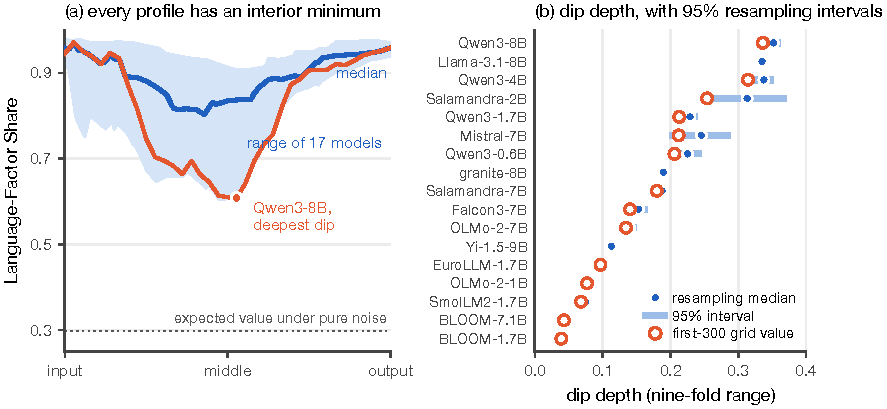
\includegraphics[width=0.66\linewidth]{fig1_lfs_profiles_17.pdf}
\end{center}
\caption{(a) LFS by relative depth for the 17 primary-set models on the
128-language, 300-sentence grid: the band is the range across models, the line
the median, and Qwen3-8B, the deepest dip, is drawn separately. Every profile has
an interior minimum with both endpoints higher, and every value lies far above
the grid's expected noise value of 0.298. (b) Dip depth, layer-0 LFS minus the minimum LFS: for the 14 models with 1,500-sentence dumps the dot is the median and the bar the 95 percent interval over 2,000 subsets of 300 sentences at the stored layers, and the hollow marker is the value on the first-300 grid (Table~\ref{tab:boot}); for the other three models only the grid value is shown; minimum layer
and minimum value per model are in Table~\ref{tab:depth_profiles}, and the
FLORES-200 replicate in Table~\ref{tab:flores}.}
\label{fig:profile}
\end{figure}

We propose such a measurement. Take $N$ sentences translated into $L$
languages, embed each of the $L \times N$ strings at one layer of a model, and
ask how the systematic variation among the resulting vectors splits between
\emph{which language} a vector came from and \emph{which sentence} it encodes.
The Language-Factor Share (LFS) is the language part of that split as a
fraction of the two systematic parts: an exact balanced two-way decomposition,
bounded, with a closed-form expected value under noise, readable at every layer.
Our contributions are the measurement, its validation, and its limits.
\textbf{(1)} We define LFS, derive its decomposition identity and its finite-grid null, and report it alongside complementary diagnostics of mapping structure, alignment tails, and representation magnitude (\S\ref{sec:method}).
\textbf{(2)} Across 33 open models we find a repeatable profile: an interior
minimum with endpoint recovery in all 17 models under the primary estimator
and all 19 under a restricted-maximum-likelihood variant, with a nine-fold
spread in dip depth that separates training recipes more than scale
(\S\ref{sec:structure}). Offsets and scale explain most of the measured cross-language
misalignment at the dip, and a multilingual average predicts each language's
representations better than an English donor.
\textbf{(3)} We test LFS against behavior after adjustment for measured
covariates. The sentence-component share at the dip layer
($1-\mathrm{LFS\text{-}VC}$) is associated with the benefit of
foreign-language context for predicting English text across 19 models and 13
families under a preregistered protocol (\S\ref{sec:validity}); it has no
clear adjusted association with pooled benchmark accuracy on 33 models, and we
discuss why that panel is a weak criterion.
\textbf{(4)} We stress-test the ratio, in the sense of \citet{naik2018stress}, with calibrated synthetic faults and
trained interventions (\S\ref{sec:stress}). LFS and retrieval-based
alignment scores are both unchanged by uniform shrinking of representation
magnitude; a trained model whose raw content variance fell twenty-fold scored
among the best on retrieval alignment. Direct minimization of LFS reverses its observational association with retrieval-tail alignment.

Every held-out prediction, fault pattern, and intervention criterion was frozen in a dated document before the corresponding run, and every failed prediction is reported; the correction ledger ships with the code. The result is a diagnostic with a clear construct, broad empirical support, target-specific behavioral relevance, and measured boundaries: not a single number that ranks models, but a decomposition read as a profile beside raw components and checks against the behavior the measure is meant to track.

\section{Related work}
\label{sec:related}

\paragraph{Language dominance and layerwise sharing.} Applying the logit lens
\citep{nostalgebraist2020lens} to non-English input often yields English
tokens at intermediate layers, prompting the claim that LLMs ``think in
English'' \citep{wendler2024llamas}; two cautions apply, that intermediate states are far from every output embedding (\S\ref{sec:structure}) and that hubness makes frequent tokens appear close to many representations \citep{radovanovic2010hubs,artetxe2017almost}. Later work reads the same layers as a shared multilingual space rather than an internal translation into English \citep{shani2025dominance,bafna2025translation}, identifies transfer neurons between shared and language-specific spaces \citep{tezuka2025transfer}, and locates language-specific neurons in the first and last layers \citep{zhao2024multilingualism,xu2025neurons,kojima2024neurons,tang2024neurons}, which become fewer after cross-lingual alignment training \citep{zhang2026neurons}. Geometry-based and decoding-based probes disagree about where languages mix \citep{bayazit2026lingua}; LFS is a geometry-based measure that reports a share rather than a latent-language label. Per-layer and instance-level descriptions of the same sharing appear in \citet{sakajo2026structural}, \citet{wilie2025interlingual}, and \citet{ravisankar2025map}.
\citet{dumas2025tongue} separate language and concept causally by activation patching. Closest to our measure, \citet{tamo2026linguamap} track per-layer language probabilities and cross-lingual similarity on three models and six languages and describe an align, reason, generate sequence; LFS measures the geometry such stages would leave behind, one number per layer with a null, on 33 models and up to 128 languages, replicated and validated, without fine-tuning; it does not itself identify functional stages.

\paragraph{Mapping between language spaces.} Non-contextual word-embedding
spaces align to a large degree under a linear or orthogonal map
\citep{conneau2018word,marchisio2021euclidean,marchisio2022isovec}, a line of work that began with lexicon induction from monolingual corpora \citep{koehn2002lexicon}, and contextual last-layer representations still admit
linear maps \citep{peng2024linear}. Language-specific information occupies a low-dimensional linear subspace that can be located per layer \citep{liang2021locating} or projected away by SVD \citep{xie2022lowrank}; \citet{zhao2025lens} use such a decomposition as a training signal, and \citet{marinov2026separability} find language concepts approximately separable as linear factors under a covariance-adjusted inner product. Our misalignment decomposition asks the same question observationally with a nested sequence of maps.

\paragraph{Intrinsic multilinguality metrics.} MEXA \citep{kargaran2024mexa}
scores whether parallel sentences retrieve each other and reports raw
correlations up to 0.9 with downstream tasks; Information Parity
\citep{tsvetkov2024ip} compares per-language compression to English; Language Ranker scores each language by representation similarity to English and relates it to pretraining share \citep{li2025ranker}; \citet{hammerl2024survey} survey alignment notions; the semantic hub hypothesis reports a shared space across languages and modalities \citep{wu2025hub}. Intrinsic scores can conflate surface form with meaning across languages \citep{poelman2026form}, and distances between language representations correlate only moderately, and inconsistently across models and layers, with transfer performance \citep{shah2024geometry}.
Representational similarity indices such as CKA \citep{kornblith2019cka} and SVCCA \citep{raghu2017svcca,kudugunta2019svcca}, layer ablations of multilingual encoders \citep{muller2021align}, and geometric analyses that read language-sensitive axes off language means \citep{chang2022geometry} describe shared structure; centering each language on its own mean makes encoder representations more language-neutral \citep{libovicky2020neutrality}. That additive picture is what LFS quantifies: how much of the two main-effect variances the language means carry, against a stated expected value, per layer.
Performance-prediction work regresses task scores on language features
\citep{lin2019langrank,xia2020nlperf}; DEPART decomposes benchmark variance into language, model, and interaction components \citep{uppadhyay2026depart}, and \citet{hu2025disparities} measure language disparities after controlling for covariates. We use the same regression form to adjust an intrinsic measure's association with behavior for measured covariates rather than to predict performance. The closest methodological relative is the neuron-level decomposition of \citet{zhao2026emotion}, who split activation probabilities in audio-language models additively into language main effects, emotion effects, interactions, and noise and report noise-corrected language-invariant shares of 0.30 to 0.59; LFS applies a decomposition of the same form to whole hidden-state vectors of text models, per layer, on 128 languages, with an analytic expected value and the tests below. Among the intrinsic measures we surveyed (Appendix~\ref{app:related}), we did not find a per-layer share of language versus matched-sentence variance that had been tested against covariate-adjusted behavior, unseen model families, and calibrated fault injection. Methodological sources for the reporting conventions and 66 further works are in Appendix~\ref{app:related}.


\section{The Language-Factor Share}
\label{sec:method}

\paragraph{Data and grid.} Let $\{s_c\}_{c=1}^{N}$ be sentences and let
$s_{\ell c}$ be the translation of sentence $c$ into language $\ell$, for
$\ell = 1, \dots, L$. At a fixed layer of a model, we run each $s_{\ell c}$,
mean-pool the token hidden states in fp32 over non-padding tokens, and obtain
one vector $\vh_{\ell c} \in \R^{D}$ per cell of a balanced $L \times N$ grid.
Each coordinate $d$ is then standardized jointly over all $LN$ cells,
$z_{\ell c d} = (h_{\ell c d} - \bar h_{\cdot\cdot d}) / s_d$, so that a few
high-variance coordinates do not dominate the sums below
\citep{timkey2021rogue}. Coordinates of very large scale are common in these models \citep{kovaleva2021outlier,sun2024massive}. Standardization is joint, never per language;
per-language standardization would remove the quantity being measured.

\paragraph{Decomposition.} Write $\bar\vz$ for the grand mean, $\bar\vz_{\ell}$
for the mean over sentences in language $\ell$, and $\bar\vz_{c}$ for the mean
over languages of sentence $c$. Define
\begin{equation}
\SSl = N \sum_{\ell=1}^{L} \lVert \bar\vz_{\ell} - \bar\vz \rVert^2, \qquad
\SSc = L \sum_{c=1}^{N} \lVert \bar\vz_{c} - \bar\vz \rVert^2, \qquad
\SSr = \sum_{\ell, c} \lVert \vz_{\ell c} - \bar\vz_{\ell} - \bar\vz_{c} + \bar\vz \rVert^2 .
\label{eq:ss}
\end{equation}
On a balanced grid the centered language means, centered sentence means, and
residuals are mutually orthogonal when summed over the grid, so
$\sum_{\ell,c} \lVert \vz_{\ell c} - \bar\vz \rVert^2 = \SSl + \SSc + \SSr$
exactly (Appendix~\ref{app:identity}). This is the vector form of a balanced
two-way analysis of variance with one observation per cell. The
Language-Factor Share is
\begin{equation}
\LFS \;=\; \frac{\SSl}{\SSl + \SSc}\,.
\label{eq:lfs}
\end{equation}
LFS is defined when $\SSl + \SSc > 0$; if both sums are zero the ratio is
undefined, not zero or one. The residual is deliberately excluded from the ratio: LFS asks how the two
\emph{systematic} main effects divide, so that a model's idiosyncratic noise
level does not masquerade as language-agnosticism. The residual, and the raw
(unstandardized) magnitudes of all three terms, are reported beside the ratio
as part of the measurement. We refer to the matched-sentence main effect as
the \emph{content component}; this is an operational proxy for structure
shared across the translations of a sentence, not a direct measure of all
semantic information. Formulas use the sentence main effect; prose uses the
content component as defined shorthand.

\paragraph{Interpretation.} $\LFS \in [0, 1]$. It equals 1 when the sentence means coincide (no sentence main effect) and 0 when the language means coincide (no language main effect); neither value implies that individual representations coincide, because the residual can remain large. LFS is a share of the two main effects, not of total variance: with main-effect sums of squares of 2 and 8 and a residual of 90, LFS is 0.20 although the sentence main effect is 8\% of the total. On a fixed grid, a lower value means a smaller language main effect relative to the sentence main effect. It does not mean language identity is absent: a linear probe on Qwen3-0.6B (24 languages, 29 layers, split by sentence) recovers language identity at $0.875$ to $0.886$ accuracy (chance $0.042$) at every layer, including the layer with the smallest share. Variance share and separability are different quantities.

\paragraph{Finite-grid null.} Under the additive model
$\vz_{\ell c} = \vC_c + \vG_\ell + \veps_{\ell c}$ with isotropic
noise of variance $\sigma^2$,
$\mathbb{E}[\SSl] = (L-1) D \sigma^2 + N \sum_\ell \lVert \vG_\ell - \bar\vG\rVert^2$
and
$\mathbb{E}[\SSc] = (N-1) D \sigma^2 + L \sum_c \lVert \vC_c - \bar\vC\rVert^2$
(Appendix~\ref{app:null}). With no language or sentence structure the expected value of LFS is
\begin{equation}
\LFS_{\mathrm{null}} = \frac{L-1}{(L-1)+(N-1)},
\label{eq:null}
\end{equation}
which is independent of $D$ but not of the grid: $0.298$ at our primary grid ($L{=}128$, $N{=}300$) and $0.078$ at $N{=}1500$. This is an expectation: a realized noise grid scatters around it, and synthetic noise across nine configurations and pseudo-language splits of real representations reproduce it to three decimals on average (Appendix~\ref{app:null}). Two consequences: measured grids lie far above this value (\S\ref{sec:structure}), and absolute values are comparable only at a fixed grid, pooling scheme, and standardization, because the expected value itself depends on $L$ and $N$. 

\paragraph{Invariances and the construct boundary.} Multiplying every entry of an analyzed grid by a common nonzero scalar multiplies both sums of squares by its square, so LFS is exactly unchanged by uniform rescaling; rescaling raw hidden states and standardizing again leaves the standardized grid unchanged up to sign, which preserves the ratio by a different route. After standardization it is unchanged by any positive diagonal rescaling of coordinates, up to the numerical stabilizer. Computed on an already standardized grid it is also unchanged by
an orthogonal rotation of that grid; rotating raw hidden states and
standardizing again changes the per-coordinate scales and hence the value
(\S\ref{sec:stress}). Scale invariance is useful for comparing structure and
dangerous when magnitude carries the failure. LFS reports the additive
language main effect: language-specific rotations, warps, and
language-by-sentence interactions are not identified separately. They enter
the residual, and they can also change the two main-effect sums of squares,
so the share records their net effect on the main effects without attributing
it. We measure the size of these components in \S\ref{sec:structure}.

\paragraph{Profile statistics.} We measure LFS at every layer, report the full curve, and summarize it by three quantities: the \emph{minimum layer}, the \emph{minimum LFS} at that layer, and the \emph{dip depth}, the layer-0 value minus the minimum LFS. A profile has an \emph{interior minimum with endpoint recovery} when the first and last layers both lie above the minimum. Layer 0 is the embedding output, so a model with $B$ blocks has $B+1$ readable layers. We do not test for a smooth symmetric curve.

\paragraph{Complementary diagnostics.} LFS needs no pivot language and no retrieval, only language membership and matched translations, so it is symmetric across languages, closed-form once representations are available, and differentiable: usable as a training monitor even though \S\ref{sec:stress} shows it is not a safe loss. It answers one question. We evaluate it alongside an external retrieval-based measure, MEXA, and complementary diagnostics of mapping structure, alignment tails, and representation magnitude on the same grid (Table~\ref{tab:family}, Appendix~\ref{app:family}), each reported separately.


\section{Experimental setup}
\label{sec:setup}

\paragraph{Parallel text.} NTREX-128 \citep{federmann2022ntrex} provides the
WMT19 news test set (1,997 sentences in 123 documents) professionally
translated into 128 languages, $n$-way parallel through English. Depth
profiles use the first 300 sentences per language and all 128 languages; a
14-model study saved 1,500-sentence representations at the dip and four
other layers for mapping, tail, and whitening analyses. NTREX is translated
from English; a native-versus-translated check on WMT19 pairs
(Appendix~\ref{app:replication}) shifts the language share by $+0.02$ to
$+0.06$ and preserves model ordering at Spearman $0.99$.

\paragraph{Models.} The primary direct-sum-of-squares set contains 17 base
models across eleven families: Qwen3 0.6B, 1.7B, 4B, 8B; OLMo-2 1B, 7B;
Mistral-7B-v0.3; EuroLLM-1.7B; BLOOM 1.7B, 7.1B; SmolLM2-1.7B; Falcon3-7B;
Salamandra 2B, 7B; granite-3.1-8B; Yi-1.5-9B; Llama-3.1-8B. Ten formed a
development grid; SmolLM2 and Falcon3 were frozen unseen families run under
pre-registered predictions; Salamandra, granite, Yi, and Llama were added
under frozen predictions after the prospective test. A second expansion set of 19 models from 13 families (Qwen2.5, XGLM, Sailor, Falcon3, SmolLM2, OLMo-2, Mistral, Tower, Occiglot, mGPT, Llama, Yi, granite; three overlap the primary set) was measured with a restricted-maximum-likelihood variant of the estimator (LFS-VC, Appendix~\ref{app:reml}); 33 unique models in total, all base checkpoints (Appendix~\ref{app:models}). The two sets were measured under different estimators, so the 33 models form one population only for the profile-shape claim. We count model families by released series (Qwen3 and Qwen2.5 separately; the continued-pretraining series Tower, Occiglot, and Sailor separately), giving 17 families across the union; the ``macro-family'' covariate below is a language family, not a model family. Table~\ref{tab:populations} lists the models, languages, sentences, estimator, and criterion of every analysis.

\paragraph{Extrinsic targets.} (i) \textbf{Belebele} \citep{bandarkar2024belebele},
four-choice reading comprehension in 122 languages, 300 questions per language, zero-shot log-likelihood scoring under one uniform prompt.
(ii) \textbf{INCLUDE} \citep{romanou2024include}, natively authored benchmarks in 30 overlapping languages, same scoring. (iii) A \textbf{content-transfer test}: whether context in another language improves the likelihood of an English continuation relative to a mismatched-context control (\S\ref{sec:validity}).

\paragraph{Confounder controls.} A metric that merely tracks how much training data a language has will correlate with any downstream score, so, following \citet{lin2019langrank,xia2020nlperf}, we fit, for each benchmark outcome $y$ on the logit scale above the chance floor,
$y = \text{model FE} + \beta_1 \log_{10}(\text{tokens}) + \beta_2\,\text{macro\mbox{-}family} + \beta_3\,\text{script} + \beta_4\,\text{fertility} + \alpha$,
with CulturaX per-language token counts \citep{nguyen2023culturax} as an exposure proxy, Glottolog macro-families \citep{hammarstrom2024glottolog}, script, and per-model tokenizer fertility, the average number of tokens per word \citep{ahia2023costs,petrov2023tokenizers}.
As a protocol check, the exposure coefficient should be positive; it is ($\beta_1 = +0.29$, SE $0.06$, $R^2 = 0.82$; Appendix~\ref{app:deflation}). Metric validity is the Spearman correlation between the
residualized metric and the residualized outcome, with cluster bootstrap
intervals by language, by model, and crossed, since languages within a model
and models within a language are not independent. The content-transfer analysis (\S\ref{sec:validity}) omits the model fixed effects, since its predictor is one value per model; its uncertainty comes from the model bootstrap.

\paragraph{Reference measure.} MEXA \citep{kargaran2024mexa}, reimplemented under the same preprocessing, is computed alongside every measure as the closest published measure and reported for reference. Alignment-at-Risk (AaR@10), the mean retrieval margin of the worst decile of sentences, is the family's tail measure (Table~\ref{tab:family}).


\section{Layerwise structure across 33 models}
\label{sec:structure}


\paragraph{Every profile dips and recovers.} All 17 direct-SS profiles and all
19 LFS-VC profiles have an interior minimum with both endpoints above it
(Table~\ref{tab:profiles}, Appendix~\ref{app:profiles}).
On the 14 models measured by both estimators, the sentence-component shares at the saved dip layer of the 1,500-sentence grids agree at Spearman $1.000$ (maximum absolute difference $0.005$; Appendix~\ref{app:reml}). The minimum lies at relative depth $0.06$ to $0.66$; most between $0.35$ and $0.6$; three (Mistral-7B and the continued-pretraining models TowerBase-7B and occiglot-7b-eu5) place a sharp minimum at layer 2 followed by a plateau. In the primary set every minimum LFS lies between $0.60$ and $0.91$, above $0.5$ and far above the expected noise value of $0.298$: even at the interior minimum the language main effect exceeds the sentence main effect on this grid, so the measure is relative. LFS-VC subtracts an estimated noise component and runs lower, so three expansion-set minima fall below $0.5$ (Table~\ref{tab:depth_profiles}; Llama-3.1-8B $0.479$ against $0.626$ under direct SS): levels are not interchangeable across estimators even where rankings agree.

\begin{table}[t]
\caption{Depth-profile summary on the 128-language, 300-sentence grid (mean pooling, joint standardization); per-model dip depths are in Figure~\ref{fig:profile}b.}
\label{tab:profiles}
\begin{center}
\small
\begin{tabular}{lcccc}
\toprule
Model set & Estimator & Models & Interior minimum & Endpoint recovery \\
\midrule
Primary grid & direct SS & 17 & 17/17 & 17/17 \\
Expansion & REML LFS-VC & 19 & 19/19 & 19/19 \\
\midrule
\bottomrule
\end{tabular}
\end{center}
\end{table}

\paragraph{Dip depth varies across families more than with size.} Within the Qwen3 series the
dip deepens monotonically with size ($0.206$, $0.213$, $0.314$, $0.336$), but
the spread across families at fixed size dwarfs that slope: Qwen3-1.7B
($0.213$) has a larger dip depth than every 7B model from another lab except Llama-3.1-8B, and BLOOM, the only deliberately balanced 46-language model in the grid, has the shallowest profile and its dip depth changes little from 1.7B to 7B ($0.039$ to $0.043$). Salamandra dips more at 2B ($0.254$) than at 7B ($0.180$) while its retrieval alignment improves, so dip depth is not a monotone scaling proxy.
The claim is descriptive: dip depth varies across model families and training histories and is not explained by parameter count alone; we do not separate data, tokenizer, and curriculum.

\paragraph{Unseen families, a second corpus, and uncertainty.} Two unseen model families were run under frozen predictions: SmolLM2-1.7B and Falcon3-7B had dip depths of $0.068$ (predicted $\le 0.15$) and $0.140$ (predicted intermediate). On FLORES-200 devtest \citep{nllb2022} (116 languages, 300 sentences), under five frozen predictions, 17 of 17 profiles recover at both endpoints and dip depths agree at Spearman $0.92$ (Appendix~\ref{app:replication}). Sentence-subsampling intervals (2,000 subsets of 300 of the 1,500 stored sentences, at the stored layers, 14 models) have 95 percent half-widths of $0.004$ to $0.020$ for 12 models and above the frozen $0.03$ bound for the two with a very early minimum (the one failed prediction of twelve; Appendix~\ref{app:replication}), and the subset ordering agrees with the grid ordering at Spearman $\geq 0.90$ in 2,000 of 2,000 subsets (median $0.996$). Six base and instruction-tuned pairs change dip depth by at most $0.01$ (Appendix~\ref{app:replication}).

\paragraph{Offsets and scale explain most measured misalignment.} At each model's
dip layer we fit a nested sequence of maps from each language into a
generalized-Procrustes consensus (a shared reference space): offset (M1), isotropic scale (M2, one scalar per language), rotation
(M3), general linear (M4), and nonlinear kernel (M5), each map credited with
its held-out reduction in reconstruction error on 20 cross-fitted splits against per-language permutation nulls (shuffled-label references); the shares are fractions of the initial held-out mapping error, not of the LFS sums of squares. Offset plus scale account for 63 to
97\% of held-out cross-language misalignment across the 14-model study
(Table~\ref{tab:budget_models});
rotation accounts for $-0.2$ to $+0.7$\% and the general linear map for
0.3 to 8\% (Figure~\ref{fig:budget}, Appendix~\ref{app:budget}). The procedure recovers injected
rotations of $0.1$ to $0.8$ rad, and additional orthogonal alignment provides
little held-out improvement under this protocol. A document-purged re-audit on Qwen3-1.7B leaves offset
plus scale at about 64\% and rotation at about 0.1\% and lowers the nonlinear
share by six points (same-document leakage in the original splits), so the nonlinear percentages may be inflated by such leakage. Per (model, language) pair, a
linear or simpler map is selected in 74\% of 1,792 cases; the 26\% nonlinear
selections concentrate in three models (Falcon3-7B, OLMo-2-1B, OLMo-2-7B).

\paragraph{A multilingual average predicts target-language representations better than an English donor.} For each target language we compare the cross-validated $R^2$ of predicting its dip-layer representations from English against predicting them from the mean of all other languages excluding English and the target; a fixed panel of 12 single-language donors is ranked as a control for the smoothness of an average. Representations are reduced to 64 principal components and predictors are standardized on the full grid before three-fold ridge fits (penalty 1), so the ridge fits, not the preprocessing, are held out. The multilingual average predicts better than English for 113 to 124 of 127 languages depending on the model (124 for most; BLOOM lowest), by a median $+0.06$ to $+0.16$ $R^2$. Among the tested donors, English is the best for 9 of 10 high-resource targets but 1 of 8 low-resource ones (areal donors take over), and its best-donor share falls from 45 to 25 of 127 across the Qwen3 series. This is consistent with a shared component that is not English-specific and whose value as a donor is resource-graded.

\section{Behavioral associations after covariate adjustment}
\label{sec:validity}

\paragraph{Pooled benchmark accuracy.} Raw correlations between intrinsic alignment and Belebele accuracy are moderate (Spearman $0.50$ to $0.54$ for MEXA and AaR on the 17-model grid) and the correlation decreases after adjustment for exposure-related covariates, to $0.19$ to $0.31$ depending on estimator. LFS itself is weaker still. On identical support (14 models, 40 languages, 522 rows) the sentence-component share $1 - \mathrm{LFS\text{-}VC}$ has covariate-adjusted Spearman $0.158$ against Belebele residual (language-cluster 95\% CI $[0.03, 0.29]$, model-cluster $[-0.02, 0.29]$); MEXA is $0.167$ $[0.09, 0.23]$. On an expanded panel of 33 models (1,740 analyzed rows over 70 languages; Table~\ref{tab:populations}) against pooled Belebele and INCLUDE accuracy, MEXA is $0.238$ $[0.18, 0.28]$, AaR $0.105$ $[0.05, 0.14]$, and $1-\mathrm{LFS\text{-}VC}$ $0.041$ $[-0.05, 0.12]$.
We do not find a clear adjusted association on this benchmark panel; the
result limits the interpretation of LFS as a general performance indicator.

Two observations qualify the panel as a criterion; pooled multiple-choice benchmarks also carry known contamination and translation artifacts \citep{deng2024contamination,gema2025mmlu}. On 30 natively authored INCLUDE languages, confounder-adjusted validity is $0.080$ $[-0.02, 0.15]$ for retrieval alignment, and the translated benchmark restricted to the same 30 languages gives $0.073$: which points to the panel's narrow resource range (log-token SD $0.92$ versus $1.67$) rather than translationese, although this comparison does not settle the question. And two independent benchmarks of the same 420 cells have adjusted residuals that correlate at only Spearman $0.315$, so the criterion itself is noisy; averaging the two benchmarks recovers a positive interval ($+0.10$ $[+0.003, +0.18]$).


\paragraph{Foreign-language context and English continuation likelihood.} We
measure whether context in another language improves the likelihood of an
English continuation, relative to a mismatched-context control. From NTREX we take an English target
sentence $s_2$ and its preceding same-document sentence $s_1$, and measure the
target's teacher-forced negative log-likelihood (its loss on the true target tokens) with no context, with $s_1$ in
each of 41 context languages, and with a length-matched \emph{wrong-document}
context in the same language. The content benefit is
$\mathrm{content}_\ell = \mathrm{NLL}_{\mathrm{mismatched},\ell} - \mathrm{NLL}_{\mathrm{matched},\ell}$,
normalized by the English benefit to give $R_{\mathrm{content},\ell}$. The mismatched control matters: wrong-document foreign text \emph{hurts} prediction in most languages, so raw context benefits understate content transfer.

A four-model pilot ($\rho = 0.84$; model-cluster CI $[-0.04, 0.91]$) could not support a model-level claim, so we froze a protocol on 19 new models from 13 families (one pair per
document from 100 documents, a deterministic minimum-cost derangement for
mismatched contexts, pinned revisions, no replacement after outcomes) and ran
it: 157,700 scored sequences, with every model showing a positive English
content effect and valid ratios in all 40 non-English languages.

\begin{table}[t]
\caption{Content transfer across 19 frozen models and 13 families (646
model-language rows, 34 common-support languages). Covariate-adjusted Spearman between
each measure and $R_{\mathrm{content}}$ with 2,000-replicate bootstrap
intervals; the LFS rows use the variance-component estimator (Appendix~\ref{app:reml}).}
\label{tab:r1}
\begin{center}
\small
\resizebox{\linewidth}{!}{%
\begin{tabular}{llccc}
\toprule
Measure & Target & $\rho$ & Model 95\% CI & Crossed 95\% CI \\
\midrule
$1-\mathrm{LFS\text{-}VC}$ (sentence-component share; one value per model) & $R_{\mathrm{content}}$ & $\mathbf{0.508}$ & $[0.19, 0.71]$ & $[0.18, 0.72]$ \\
MEXA (reference) & $R_{\mathrm{content}}$ & $0.591$ & $[0.33, 0.82]$ & $[0.31, 0.82]$ \\
AaR@10 (tail measure) & $R_{\mathrm{content}}$ & $0.443$ & $[0.09, 0.71]$ & $[0.08, 0.72]$ \\
$1-\mathrm{LFS\text{-}VC}$ & raw content & $0.620$ & $[0.34, 0.77]$ & $[0.35, 0.78]$ \\
\midrule
\multicolumn{5}{l}{Model level ($n{=}19$): Spearman of $1-\mathrm{LFS\text{-}VC}$ vs.\ median $R_{\mathrm{content}}$, $0.770$ $[0.44, 0.94]$.} \\
\multicolumn{5}{l}{Leave-one-family-out $\rho$: $0.44$ to $0.60$, all positive; family-bootstrap CI $[0.24, 0.76]$.} \\
\bottomrule
\end{tabular}}
\end{center}
\end{table}

Table~\ref{tab:r1} gives the result. The association remains positive in the
model-level and family-deletion sensitivity analyses: $\rho = 0.508$ with a model-bootstrap interval that excludes
zero, positive under every leave-one-family-out deletion, and $0.770$ at the
model level. It is smaller than the pilot estimate, as expected for an estimate selected on a small support. MEXA has a larger point estimate on the same test with overlapping intervals; the two measure different things (a variance partition versus nearest-neighbor discriminability), and the result here is that a structural measure which never looks at nearest neighbors is associated with a context-use behavior measured at generation time (Figure~\ref{fig:r1}).

\begin{figure}[t]
\begin{center}
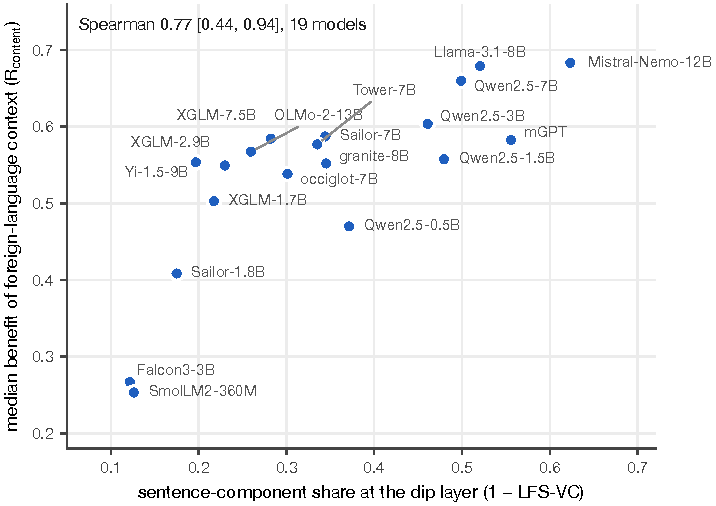
\includegraphics[width=0.62\linewidth]{fig_r1_model_level.pdf}
\end{center}
\caption{Model-level view of the content-transfer result: each point is one of
the 19 frozen models, placed by $1-\mathrm{LFS\text{-}VC}$ at the dip
layer and its median normalized content benefit over 34 languages. The
annotation is the unadjusted model-level Spearman correlation ($0.77$); the
covariate-adjusted value reported in the text is $0.51$. Thin gray lines are
label connectors only.}
\label{fig:r1}
\end{figure}

\section{Stress tests: where the ratio fails}
\label{sec:stress}

\paragraph{Uniform shrinking is invisible to every scale-invariant measure.} Any statistic that is unchanged when all representations are multiplied by the same nonzero constant cannot register uniform shrinking of representation magnitude. Nonzero uniform scaling changes neither the rank nor the relative eigenvalue spectrum, so this is distinct from the dimensional collapse studied in contrastive learning \citep{jing2022collapse,wang2020uniformity}, in which dimensions are lost. In a 14-model analytic sweep of the full measure suite, 3,414 of 3,416 invariance checks under uniform and (after standardization) diagonal rescaling pass; the two exceptions are numerical-tolerance flags below $10^{-7}$ on AaR and the mean margin for one model. Shrinking the non-English languages toward the global centroid by 30, 60, or 90 percent (test-suite condition I8b, three models) moves LFS by only $-0.04$ to $+0.05$ and leaves MEXA within 0.01 of its value, because retrieval is order-based; only the content-variance preservation check fires (CVP: within-language variance across sentences, averaged over the perturbed languages, relative to the reference), returning $(1-m)^2$ to three decimals for shrinkage $m$, as predicted before the run.

\paragraph{A trained model shows this pattern.} The word-level alignment objective proposed in the alignment literature \citep{cao2020alignment}, a squared difference
between representations of dictionary-linked words in a sentence and its
translation, is globally minimized at $\vh = 0$. Fine-tuning Qwen3-0.6B with
it for 400 steps (three seeds) shrank mean representation norm from 451 to 42
and raw content variance (the same within-language variance, unstandardized) at the measured layer from 13,791 to 699, a factor of twenty (Figure~\ref{fig:ratio}). LFS moved from $0.445$ to $0.493$. MEXA rose by $+0.09$ over the LM-only control for the shrunk model, and the shrinking conditions had the highest retrieval and tail scores as a group, while a cosine variant that does not shrink (CVP $1.000$) gained nothing. Norms and raw content variance fell substantially while retrieval-based scores rose; the raw components separate the shrunk and unshrunk models twenty-fold, and the ratio divides that difference out. Two facts bound the interpretation: the shrunk model matched its control on a 40-language Belebele panel ($0.395$ versus $0.390$), and conditions that did lose ability (about six points) had unchanged geometry. The check flags representation change, not demonstrated capability loss.


\paragraph{Observational associations reverse under intervention.} Across pretrained models, a deeper dip accompanies better retrieval alignment; across 18 condition-seed points from six experimental conditions, LFS and tail alignment were positively correlated (Pearson $+0.92$): the objectives that drove LFS down drove tail alignment down with it. Fine-tuning with LFS itself as a loss doubled the dip in 400 steps while aggregate Belebele fell 2.9 points against the control's 1.7. LFS is a measurement, not a safe objective; the variance-preservation penalty tested here, a squared hinge on the aggregate content-variance ratio, saturated at every weight tested (1 to 1{,}000) and did not prevent the contraction under this setup.


\paragraph{Measurement dependence.} Pooling choice changes absolute dip depth by $0.13$ to $0.20$ while the cross-model ordering changes by at most one adjacent transposition; ZCA whitening changes the ordering substantially (Spearman $0.45$ against the raw-coordinate ordering; Appendix~\ref{app:measdep}).

\section{Limitations}
\label{sec:limitations}

LFS is a two-way main-effect share: it captures additive language structure, excludes the interaction residual by design, and is blind to common scale; absolute values are comparable only at fixed grid, pooling, and standardization. Validation lives in the translated-news domain except for the INCLUDE and WMT19 controls; the behavioral association is target-specific (content transfer yes, pooled benchmarks no); and the cross-model associations are observational: the only controlled interventions are the training conditions on one 0.6B model, which show what the measures do under those objectives and do not identify causes of the cross-model pattern.

\section{Conclusion}
\label{sec:conclusion}
Across 33 open models the language main effect is high at the input, lowest at an interior layer, and high again at the output; dip depth varies nine-fold across the primary models and is not explained by parameter count alone; offsets and scale explain most of the remaining cross-language misalignment; a multilingual average predicts most target languages better than an English donor; and the sentence-component share is associated with the benefit of foreign-language context for predicting English text. Read as a profile beside $\SSl$, $\SSc$, the residual, and the norm, with a behavioral check chosen for the question, LFS is a diagnostic; as a score or a loss it becomes a Goodhart target \citep{gao2023scaling}.

\subsubsection*{Reproducibility statement}
Representation grids derive from public NTREX-128 and FLORES-200 text and public checkpoints (base models, plus the instruction-tuned checkpoints of the control comparison) with pinned revisions (Appendix~\ref{app:models}). The estimator
is defined in Eqs.~\ref{eq:ss} and \ref{eq:lfs}; Appendix~\ref{app:identity}
proves the decomposition identity and Appendix~\ref{app:null} the finite-grid
null. Every main number is mapped to its producing script, input hashes,
and job identifier in a claims ledger included with the supplementary code,
together with the frozen preregistration documents and the discrepancy ledger
of every correction made during the project. Predictions for the unseen
model families, the synthetic fault test suite, the intervention conditions,
and the 19-model content-transfer expansion were frozen in dated documents
before the corresponding runs, and every failed prediction is reported. The anonymized code repository link will be added at submission.

\subsubsection*{Ethics statement}
This work analyzes publicly released base language models on public
benchmark text and involves no human subjects. Its aim is to improve the
evaluation of multilingual models so that non-English users are served
better; a risk we note is that any scalar multilinguality score can be gamed,
which is a central finding of the paper.

\subsubsection*{AI use statement}
% Authors confirm every clause before submission.
In this work, we used generative AI assistants for implementing and reviewing analysis code, designing and checking analysis protocols, interpreting results, drafting and editing text, producing figures, and organizing the literature review. We have not used generative AI tools for generating
synthetic datasets or for producing any reported measurement; all numbers in
this paper were computed by the released scripts on the stated inputs and
verified against saved artifacts by the authors. Mathematical claims
(the decomposition identity and the finite-grid null) were checked by hand and
by unit tests. We take responsibility for the final content of this work,
including text, claims or artifacts produced with the aid of generative AI.

\bibliography{references}
\bibliographystyle{iclr2027_conference}

\appendix
\section{Decomposition identity}
\label{app:identity}
\begin{figure}[h]
\begin{center}
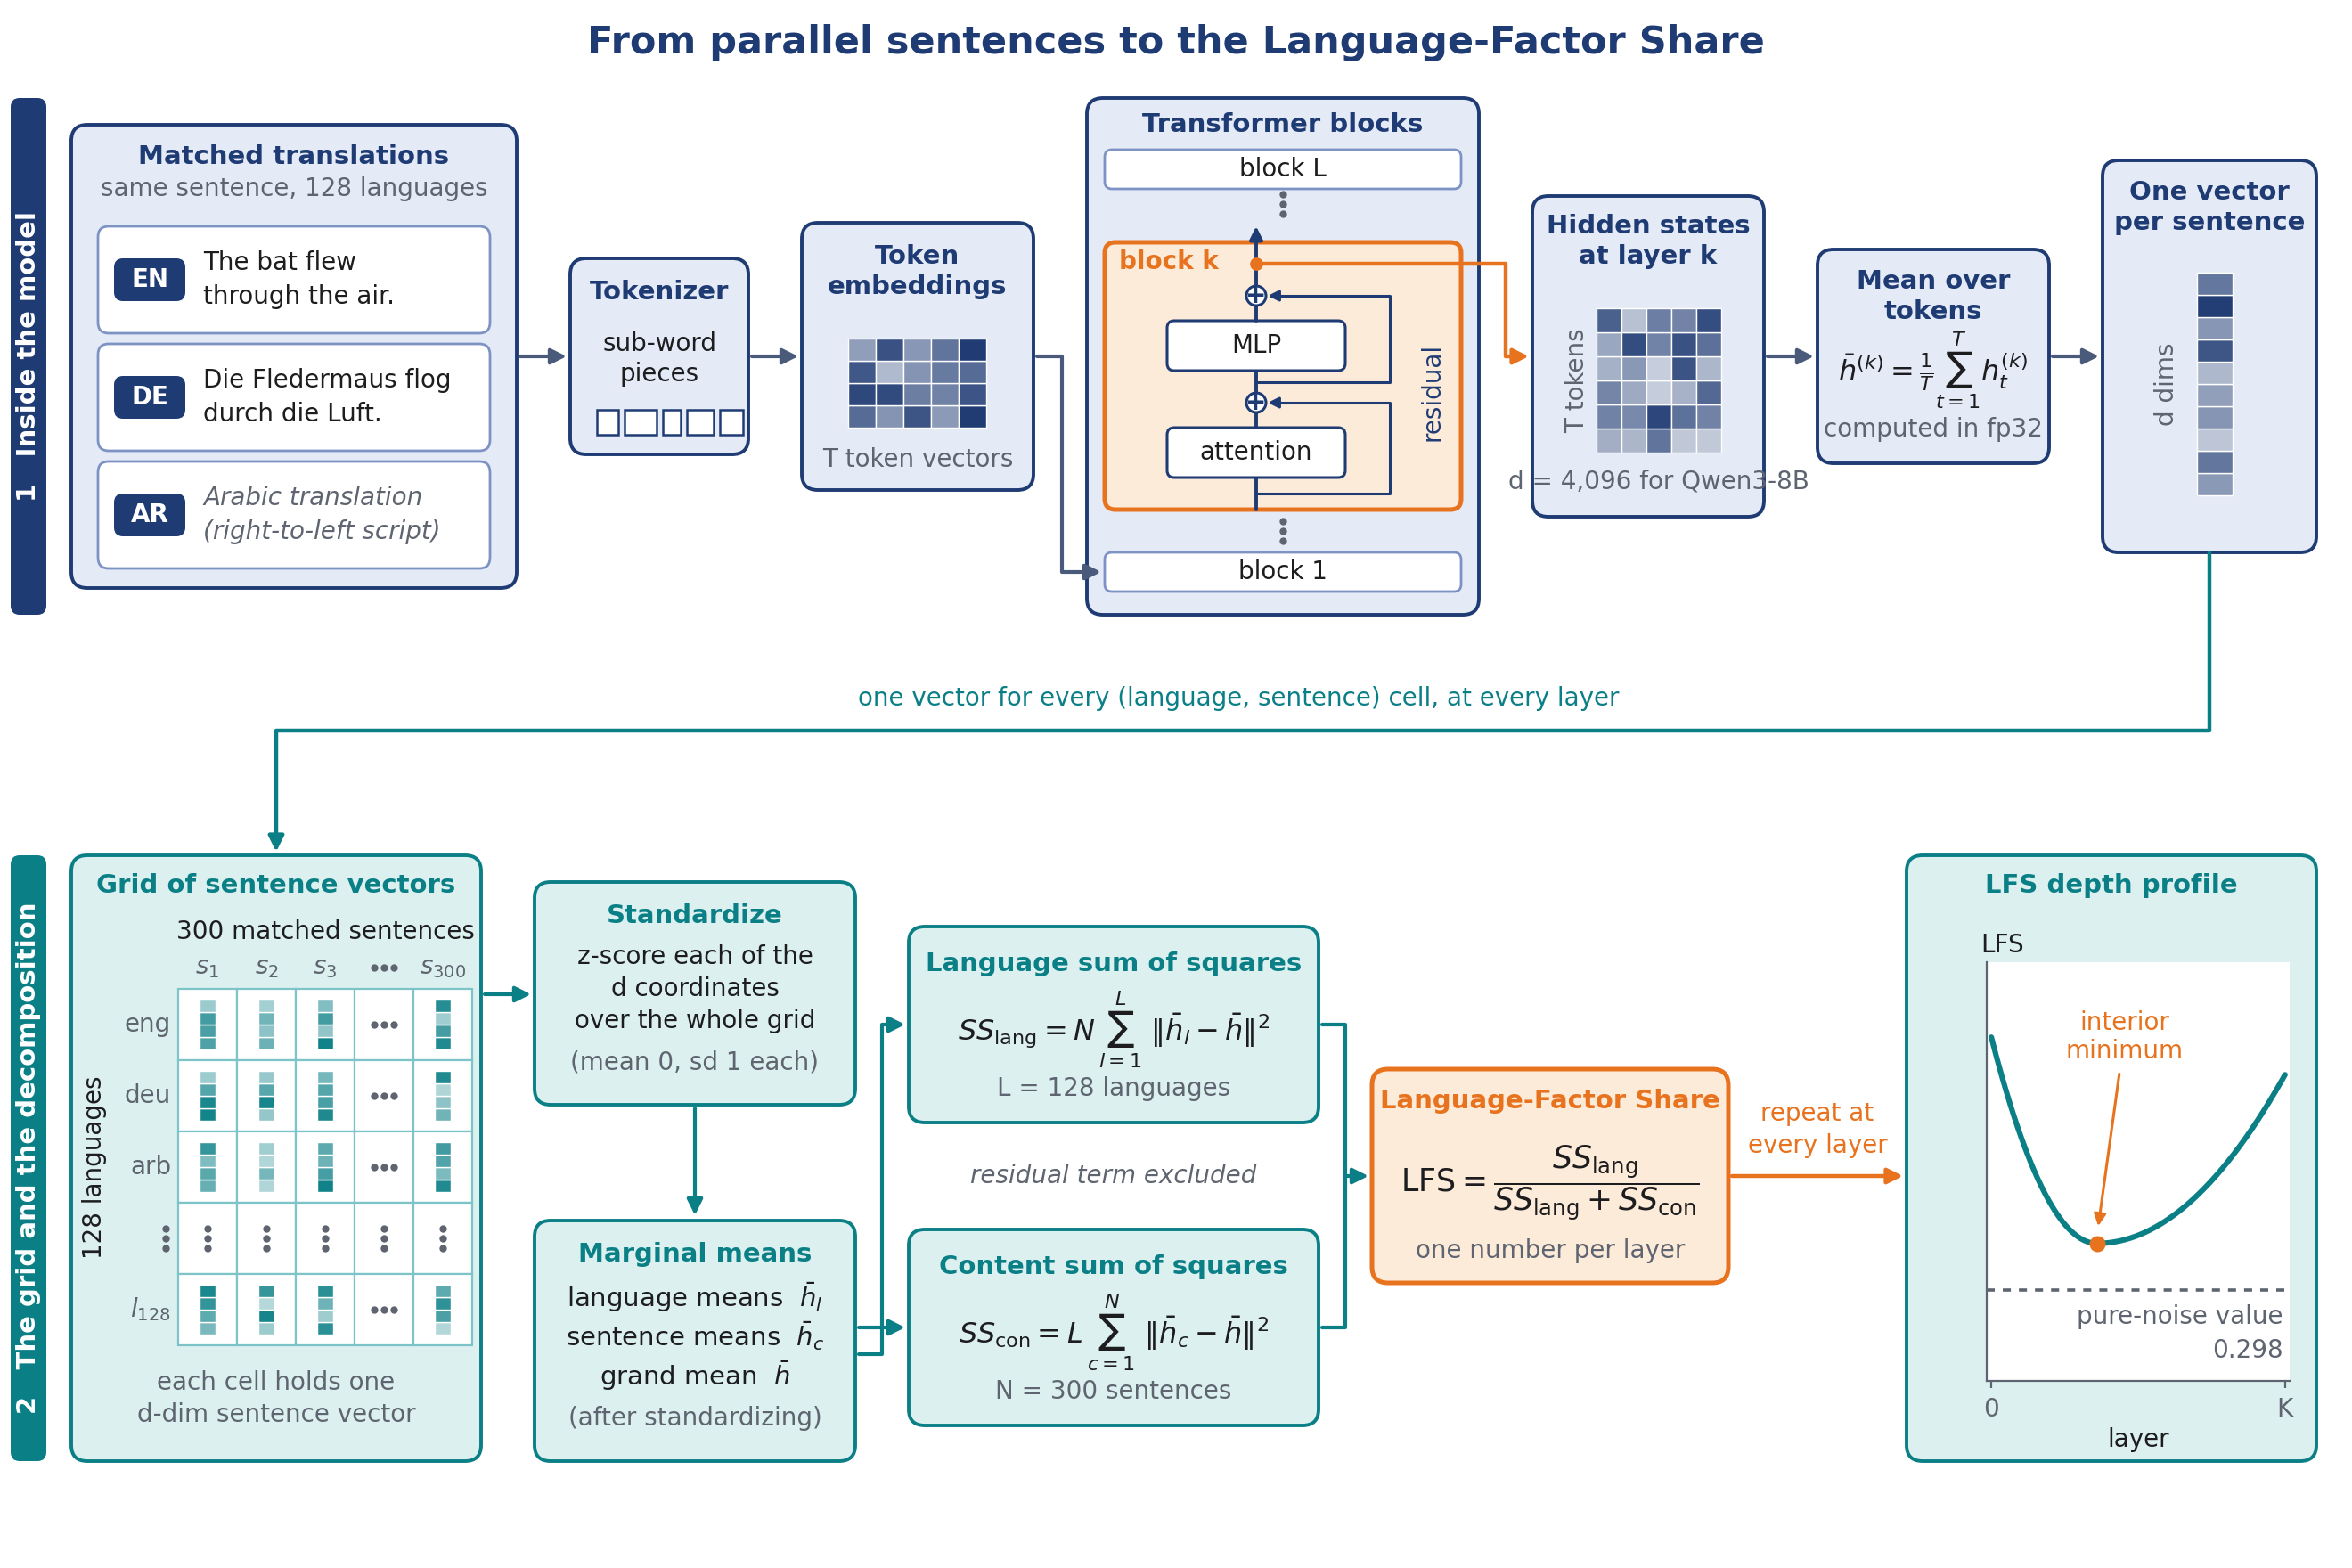
\includegraphics[width=\linewidth]{fig22_pipeline_diagram.png}
\end{center}
\caption{Schematic of the measurement. Top: one sentence per language is tokenized, embedded, and carried through the Transformer blocks; hidden states at layer $k$ are mean-pooled in fp32 into one vector per sentence. Bottom: the vectors form a languages-by-sentences grid; each coordinate is standardized over the grid; language means, sentence means, and the grand mean give $\SSl$ and $\SSc$, whose ratio is LFS at that layer; repeating over layers gives the depth profile.}
\label{fig:pipeline}
\end{figure}
Let $a_\ell = \bar\vz_\ell - \bar\vz$, $b_c = \bar\vz_c - \bar\vz$, and
$r_{\ell c} = \vz_{\ell c} - \bar\vz_\ell - \bar\vz_c + \bar\vz$, so that
$\vz_{\ell c} - \bar\vz = a_\ell + b_c + r_{\ell c}$. On a balanced grid
$\sum_\ell a_\ell = 0$, $\sum_c b_c = 0$, $\sum_c r_{\ell c} = 0$ for every
$\ell$, and $\sum_\ell r_{\ell c} = 0$ for every $c$. Expanding
$\sum_{\ell c} \lVert a_\ell + b_c + r_{\ell c}\rVert^2$, the cross term
$2\sum_{\ell c} a_\ell^\top b_c = 2 (\sum_\ell a_\ell)^\top(\sum_c b_c) = 0$,
the cross term $2\sum_{\ell c} a_\ell^\top r_{\ell c} = 2\sum_\ell a_\ell^\top
(\sum_c r_{\ell c}) = 0$, and likewise for $b_c$. Hence
$\sum_{\ell c}\lVert \vz_{\ell c} - \bar\vz\rVert^2 = N\sum_\ell \lVert
a_\ell\rVert^2 + L \sum_c \lVert b_c \rVert^2 + \sum_{\ell c}\lVert r_{\ell c}
\rVert^2 = \SSl + \SSc + \SSr$. The multipliers $N$ and $L$ arise because each
language mean is repeated across $N$ sentences and each sentence mean across
$L$ languages.

\section{Finite-grid null}
\label{app:null}
Under $\vz_{\ell c} = \vC_c + \vG_\ell + \veps_{\ell c}$ with
i.i.d.\ isotropic noise of variance $\sigma^2$ per coordinate, the language
means are $\bar\vz_\ell = \vG_\ell + \bar\vC + \bar{\veps}_{\ell\cdot}$,
and $\mathbb{E}\,N\sum_\ell \lVert \bar{\veps}_{\ell\cdot} -
\bar{\veps}\rVert^2 = (L-1) D \sigma^2$ by the usual
between-groups degrees of freedom. Thus
$\mathbb{E}[\SSl] = (L-1)D\sigma^2 + N\sum_\ell\lVert \vG_\ell - \bar\vG\rVert^2$
and symmetrically
$\mathbb{E}[\SSc] = (N-1)D\sigma^2 + L\sum_c\lVert \vC_c - \bar\vC\rVert^2$.
With no structure, $\SSl$ and $\SSc$ are independent scaled chi-square variables with $(L-1)D$ and $(N-1)D$ degrees of freedom (Cochran's theorem applied to the orthogonal projections of a Gaussian grid), so $\LFS$ is Beta-distributed with expectation exactly $(L-1)/(L+N-2)$; the expectation of the ratio equals the ratio of expectations only because of this independence. Empirical coordinate standardization makes the entries weakly dependent, so on standardized grids the value is approximate, which the synthetic checks below cover. The null is not a lower bound, since strong concept structure with weak language
structure drives LFS below it. Synthetic checks across
$L\in[2,128]$, $N\in[50,3000]$, $D\in[64,1024]$ and pseudo-language splits of
real representations ($0.0015$ measured against $0.00143$ predicted at
$(2,700)$; $0.0849$ against $0.0846$ at $(12,120)$) confirm the formula.
LFS is nearly but not exactly size-independent: on fixed language sets it moves by $-0.006$ to $-0.010$ from $N{=}100$ to $N{=}1000$, against $-0.065$ to $-0.125$ for a retrieval-based score on the same draws.

\section{The REML variant (LFS-VC)}
\label{app:reml}
Treating Eq.~\ref{eq:ss} as a balanced two-way crossed random-effects layout
with one observation per cell, the expected mean squares are
$\mathbb{E}[\mathrm{MS}_L] = \sigma_E^2 + N\sigma_L^2$,
$\mathbb{E}[\mathrm{MS}_C] = \sigma_E^2 + L\sigma_C^2$,
$\mathbb{E}[\mathrm{MS}_E] = \sigma_E^2$, giving per-coordinate interior estimates $\hat\sigma_L^2 = (\mathrm{MS}_L - \mathrm{MS}_E)/N$ and $\hat\sigma_C^2 = (\mathrm{MS}_C - \mathrm{MS}_E)/L$. Non-negativity is enforced by refitting on the boundary: a negative component is set to zero, the error is re-pooled with that effect's sum of squares, and the other component is re-estimated against the pooled error; when both initial estimates are negative the implementation sets both to zero, which is not always the constrained optimum. In every saved fit behind this paper (104 stored fits, including all 14 same-support grids and all training conditions) no coordinate produced a negative estimate, so this branch never affected a reported value. Summing over coordinates,
$\mathrm{LFS\mbox{-}VC} = \sigma_L^2/(\sigma_L^2 + \sigma_C^2)$. The two
estimators are mathematically distinct; on 14 shared models the sentence-component shares at the saved dip layer agree at Spearman $1.000$ (maximum absolute difference $0.005$), but levels differ because the variance components subtract the residual mean square and divide by $N$ or $L$ rather than sharing raw sums of squares (Llama-3.1-8B minimum $0.626$ under direct SS
against $0.479$ under LFS-VC). Direct SS is primary for the profile results;
the expansion set and the content-transfer analysis use LFS-VC and are labeled
as such throughout. A same-protocol re-measurement of the 19 expansion models
with the direct-SS estimator has not been run; until it is, the two estimators
are reported separately and never pooled.

\section{Misalignment decomposition}
\label{app:budget}
\begin{figure}[h]
\begin{center}
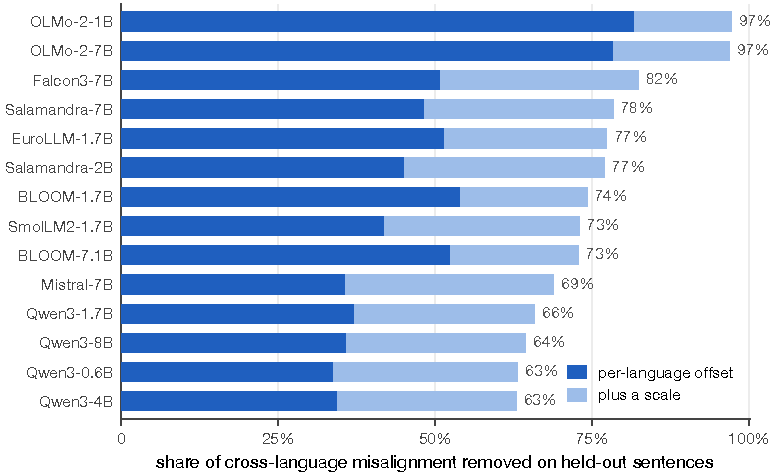
\includegraphics[width=0.8\linewidth]{fig15_budget_composition.pdf}
\end{center}
\caption{Misalignment decomposition at the dip layer for the 14-model study
($N{=}1500$, common rank 64). Additive offset and isotropic scale dominate
every model; the rotation share, given per model in Table~\ref{tab:budget_models},
never exceeds 0.7\%.}
\label{fig:budget}
\end{figure}
Per-model held-out shares at the common rank are given in Table~\ref{tab:budget_models}.
% ---- table budget_models (inlined) ----
\begin{table}[h]
\caption{Misalignment decomposition at each model's dip layer for the 14-model study: mean held-out error-reduction share across 128 languages at the common rank 64, for the nested maps offset (M1), isotropic scale (M2), rotation (M3), general linear (M4), and nonlinear kernel (M5). A negative nonlinear share is held-out overfitting of the kernel map at 300 sentences, reported as measured.}
\label{tab:budget_models}
\begin{center}\small
\begin{tabular}{lrrrrrrr}
\toprule
Model & Dip layer & Offset & Scale & Rotation & Linear & Nonlinear & Offset$+$scale \\
\midrule
BLOOM-1.7B & 14 & 54.1\% & 20.1\% & 0.6\% & 5.0\% & $-$6.3\% & 74.2\% \\
BLOOM-7.1B & 17 & 52.4\% & 20.5\% & 0.7\% & 5.2\% & $-$7.0\% & 72.9\% \\
EuroLLM-1.7B & 14 & 51.5\% & 25.8\% & 0.4\% & 3.6\% & $-$1.7\% & 77.4\% \\
Falcon3-7B & 13 & 50.9\% & 31.4\% & 0.1\% & 3.0\% & 1.1\% & 82.3\% \\
Mistral-7B-v0.3 & 2 & 35.7\% & 33.2\% & 0.0\% & 3.4\% & $-$10.5\% & 68.9\% \\
OLMo-2-1B & 9 & 81.8\% & 15.4\% & $-$0.2\% & 0.3\% & 0.5\% & 97.2\% \\
OLMo-2-7B & 12 & 78.4\% & 18.5\% & $-$0.2\% & 0.4\% & 0.7\% & 96.9\% \\
Qwen3-0.6B & 8 & 33.8\% & 29.4\% & 0.0\% & 4.1\% & $-$12.4\% & 63.2\% \\
Qwen3-1.7B & 13 & 37.2\% & 28.6\% & 0.1\% & 4.2\% & $-$10.8\% & 65.8\% \\
Qwen3-4B & 17 & 34.5\% & 28.4\% & 0.1\% & 8.0\% & $-$12.1\% & 62.9\% \\
Qwen3-8B & 19 & 35.9\% & 28.5\% & 0.1\% & 7.3\% & $-$9.5\% & 64.4\% \\
Salamandra-2B & 6 & 45.2\% & 31.8\% & $-$0.1\% & 2.3\% & $-$1.2\% & 77.0\% \\
Salamandra-7B & 18 & 48.2\% & 30.1\% & 0.1\% & 1.8\% & 1.2\% & 78.3\% \\
SmolLM2-1.7B & 15 & 42.0\% & 31.0\% & 0.1\% & 2.1\% & $-$5.3\% & 73.0\% \\
\bottomrule
\end{tabular}
\end{center}
\end{table}


\section{Models and revisions}
\label{app:models}
The 19 expansion models were run at the pinned Hugging Face revisions below. The 17 primary-set models are listed in Table~\ref{tab:depth_profiles}; their cached snapshot revisions are recorded in the run manifests and will be listed in the camera-ready.
% ---- table models_a9 (inlined) ----
\begin{center}\scriptsize
\begin{tabular}{llll}
\toprule
Tag & Hugging Face id & Revision (first 12) & Family \\
\midrule
Qwen2.5-0.5B & Qwen/Qwen2.5-0.5B & \texttt{060db6499f32} & Qwen2.5 \\
Qwen2.5-1.5B & Qwen/Qwen2.5-1.5B & \texttt{8faed761d45a} & Qwen2.5 \\
Qwen2.5-3B & Qwen/Qwen2.5-3B & \texttt{3aab1f1954e9} & Qwen2.5 \\
Qwen2.5-7B & Qwen/Qwen2.5-7B & \texttt{d14972939875} & Qwen2.5 \\
xglm-1.7B & facebook/xglm-1.7B & \texttt{d23a5e8e2164} & XGLM \\
xglm-2.9B & facebook/xglm-2.9B & \texttt{33c659ae27de} & XGLM \\
xglm-7.5B & facebook/xglm-7.5B & \texttt{732d59308a84} & XGLM \\
mGPT & ai-forever/mGPT & \texttt{40897bd7c8b4} & mGPT \\
OLMo-2-1124-13B & allenai/OLMo-2-1124-13B & \texttt{3fefddc1bf18} & OLMo-2 \\
granite-3.1-8b-base & ibm-granite/granite-3.1-8b-base & \texttt{39975ba90995} & Granite \\
Yi-1.5-9B & 01-ai/Yi-1.5-9B & \texttt{80d5471b1eae} & Yi-1.5 \\
TowerBase-7B & Unbabel/TowerBase-7B-v0.1 & \texttt{bd59c10d7600} & Tower \\
occiglot-7b-eu5 & occiglot/occiglot-7b-eu5 & \texttt{72d8b932ce09} & Occiglot \\
Sailor-1.8B & sail/Sailor-1.8B & \texttt{c687a96d5c3e} & Sailor \\
Sailor-7B & sail/Sailor-7B & \texttt{b8b49a0f0207} & Sailor \\
Llama-3.1-8B & meta-llama/Llama-3.1-8B & \texttt{d04e592bb4f6} & Llama-3.1 \\
SmolLM2-360M & HuggingFaceTB/SmolLM2-360M & \texttt{f8027fd0eaee} & SmolLM2 \\
Falcon3-3B-Base & tiiuae/Falcon3-3B-Base & \texttt{092c29e3114f} & Falcon3 \\
Mistral-Nemo-Base-2407 & mistralai/Mistral-Nemo-Base-2407 & \texttt{a4477a2f9779} & Mistral \\
\bottomrule
\end{tabular}
\end{center}

\begin{table}[h]\caption{Analysis populations. Each row lists what a result in the main text was computed on.}\label{tab:populations}
\begin{center}\small
\resizebox{\linewidth}{!}{%
\begin{tabular}{llllll}
\toprule
Analysis & Models & Languages & Sentences & Estimator & Criterion or output \\
\midrule
Depth profiles, primary (Table~\ref{tab:profiles}) & 17 & 128 & 300 & direct SS & minimum layer, minimum LFS, dip depth \\
Depth profiles, expansion & 19 & 128 & 300 & LFS-VC & same \\
FLORES-200 replication & 17 & 116 & 300 & direct SS & same \\
Sentence-subsampling intervals & 14 & 128 & 300 of 1,500 & direct SS & dip depth at fixed layers \\
Misalignment decomposition & 14 & 128 & 1,500 & nested maps M0--M5 & held-out error reduction \\
English donor vs.\ multilingual average & 17 & 127 targets & 300 & ridge $R^2$ & held-out $R^2$ \\
Content transfer & 19 & 41 (34 common support) & 100 pairs & $1-$LFS-VC & $R_{\mathrm{content}}$ \\
Pooled benchmark panel & 33 & 70 of 73 & 1,740 of 2,001 rows & $1-$LFS-VC & pooled Belebele and INCLUDE residual \\
Training conditions & Qwen3-0.6B & 128 & 300 & direct SS & components, MEXA, AaR, CVP \\
\bottomrule
\end{tabular}}
\end{center}
\end{table}

\section{Per-model depth profiles}
\label{app:profiles}
Table~\ref{tab:depth_profiles} lists every audited profile. Dip depth is the first-layer value minus the minimum.
\begin{table}[h]\caption{All 36 audited depth profiles (17 direct-SS, 19 REML LFS-VC; three models appear in both).}\label{tab:depth_profiles}
% ---- table depth_profiles (inlined) ----
\begin{center}\scriptsize
\begin{tabular}{lrrrrrrr}
\toprule
Model & Layers & Min.\ layer & Rel.\ depth & First & Minimum & Last & Dip depth \\
\midrule
\multicolumn{8}{l}{\emph{Primary set, direct sums of squares}} \\
Qwen3-8B-Base & 37 & 19 & 0.53 & 0.945 & 0.608 & 0.958 & 0.336 \\
Llama-3.1-8B & 33 & 14 & 0.44 & 0.961 & 0.626 & 0.936 & 0.335 \\
Qwen3-4B-Base & 37 & 17 & 0.47 & 0.916 & 0.602 & 0.956 & 0.314 \\
salamandra-2b & 25 & 6 & 0.25 & 0.966 & 0.712 & 0.935 & 0.254 \\
Qwen3-1.7B-Base & 29 & 13 & 0.46 & 0.927 & 0.715 & 0.960 & 0.213 \\
Mistral-7B-v0.3 & 33 & 2 & 0.06 & 0.956 & 0.744 & 0.963 & 0.212 \\
Qwen3-0.6B-Base & 29 & 8 & 0.29 & 0.933 & 0.728 & 0.958 & 0.206 \\
granite-3.1-8b-base & 41 & 14 & 0.35 & 0.898 & 0.709 & 0.969 & 0.190 \\
salamandra-7b & 33 & 18 & 0.56 & 0.963 & 0.784 & 0.938 & 0.180 \\
Falcon3-7B-Base & 29 & 13 & 0.46 & 0.967 & 0.826 & 0.962 & 0.140 \\
OLMo-2-1124-7B & 33 & 12 & 0.38 & 0.981 & 0.846 & 0.956 & 0.135 \\
Yi-1.5-9B & 49 & 20 & 0.42 & 0.973 & 0.860 & 0.963 & 0.113 \\
EuroLLM-1.7B & 25 & 14 & 0.58 & 0.951 & 0.854 & 0.937 & 0.097 \\
OLMo-2-0425-1B & 17 & 9 & 0.56 & 0.980 & 0.903 & 0.958 & 0.077 \\
SmolLM2-1.7B & 25 & 15 & 0.62 & 0.972 & 0.904 & 0.973 & 0.068 \\
bloom-7b1 & 31 & 17 & 0.57 & 0.927 & 0.884 & 0.953 & 0.043 \\
bloom-1b7 & 25 & 14 & 0.58 & 0.938 & 0.899 & 0.948 & 0.039 \\
\multicolumn{8}{l}{\emph{Expansion set, REML LFS-VC}} \\
Mistral-Nemo-Base-2407 & 41 & 13 & 0.33 & 0.907 & 0.377 & 0.822 & 0.530 \\
mGPT & 25 & 12 & 0.50 & 0.950 & 0.444 & 0.767 & 0.506 \\
Llama-3.1-8B & 33 & 14 & 0.44 & 0.966 & 0.479 & 0.883 & 0.487 \\
Qwen2.5-7B & 29 & 14 & 0.50 & 0.953 & 0.501 & 0.911 & 0.452 \\
Qwen2.5-1.5B & 29 & 15 & 0.54 & 0.923 & 0.521 & 0.939 & 0.403 \\
Qwen2.5-3B & 37 & 19 & 0.53 & 0.924 & 0.539 & 0.932 & 0.385 \\
TowerBase-7B & 33 & 2 & 0.06 & 0.974 & 0.665 & 0.943 & 0.309 \\
Qwen2.5-0.5B & 25 & 11 & 0.46 & 0.909 & 0.629 & 0.935 & 0.280 \\
Sailor-7B & 33 & 14 & 0.44 & 0.934 & 0.656 & 0.954 & 0.279 \\
occiglot-7b-eu5 & 33 & 2 & 0.06 & 0.969 & 0.699 & 0.968 & 0.270 \\
granite-3.1-8b-base & 41 & 15 & 0.38 & 0.911 & 0.655 & 0.958 & 0.256 \\
OLMo-2-1124-13B & 41 & 19 & 0.47 & 0.985 & 0.740 & 0.916 & 0.244 \\
Yi-1.5-9B & 49 & 20 & 0.42 & 0.984 & 0.803 & 0.950 & 0.181 \\
xglm-2.9B & 49 & 21 & 0.44 & 0.936 & 0.770 & 0.981 & 0.166 \\
xglm-1.7B & 25 & 13 & 0.54 & 0.944 & 0.783 & 0.987 & 0.161 \\
Sailor-1.8B & 25 & 11 & 0.46 & 0.951 & 0.825 & 0.956 & 0.126 \\
SmolLM2-360M & 33 & 20 & 0.62 & 0.979 & 0.874 & 0.983 & 0.106 \\
Falcon3-3B-Base & 23 & 11 & 0.50 & 0.979 & 0.878 & 0.972 & 0.101 \\
xglm-7.5B & 33 & 21 & 0.66 & 0.790 & 0.718 & 0.850 & 0.072 \\
\bottomrule
\end{tabular}
\end{center}

\end{table}

\section{Confounder-adjustment regression details}
\label{app:deflation}
The adjustment regresses each benchmark outcome (on the logit scale above the chance floor) on model fixed effects, $\log_{10}$ CulturaX tokens, Glottolog macro-family, script, and tokenizer fertility, with cluster-robust standard errors by language. On the 17-model grid (1,241 model-language rows) the fit has $R^2 = 0.824$; the token coefficient is $+0.286$ (SE $0.059$, $z = 4.8$) and the fertility coefficient $-0.103$ (SE $0.022$); no macro-family or script dummy is individually significant. An earlier development-grid run (10 models, 1,173 rows) gave a token coefficient of $+0.267$ (SE $0.051$) and $R^2 = 0.86$; the main text reports the 17-model values. Rows lacking a token count or a fertility value are dropped before fitting, which is why the analyzed row counts in \S\ref{sec:validity} are below the panel sizes. The residual $\alpha$ from this fit is the adjusted outcome; the content-transfer outcome, $R_{\mathrm{content}}$, is residualized on its raw scale by ordinary least squares on the same covariates without model fixed effects.

\section{Content-transfer protocol}
\label{app:r1}
The candidate measure is one frozen number per model: $q_L = 1 - \mathrm{LFS\text{-}VC}$ at the dip layer, taken from the expansion-set estimator. On the 14 models measured by both estimators, the sentence-component shares at the saved dip layer of the 1,500-sentence grids agree at Spearman 1.000 (Appendix~\ref{app:reml}); that comparison uses a different grid from the 300-sentence profiles and does not establish that the two estimators give equivalent values on this set, which is why this result is reported as an LFS-VC result throughout. Because it is constant within a model, the 646-row correlation reflects between-model variation with languages as repeated measures; the model-bootstrap interval and the model-level Spearman of $0.770$ over 19 models are the statements that account for this.
Pairs: for each NTREX document, the first adjacent pair whose context sentence has at least five English words and whose target has 8 to 45 words; the first 100 distinct documents; a deterministic minimum-cost derangement assigns each pair a wrong-document context of matched English length (mean absolute mismatch 0.34 words). Scoring: teacher-forced fp32 NLL over target tokens only, context and target separated by a newline; 41 context languages; 8,300 sequences per model. Ten models initially exceeded a tokenizer-length ceiling and were rerun with a 1,024-token and then a 2,048-token limit; no example, revision, or scoring rule changed. Table~\ref{tab:r1_models} gives the per-model values.

\paragraph{Attention (secondary result).} On the same pairs (Qwen3-0.6B, 41 languages, frozen predictions), matched context draws more attention than mismatched in 41 of 41 languages, peaking just below the LFS minimum, and content attention tracks alignment after confounder adjustment ($0.53$ $[0.27, 0.73]$); the attention-to-behavior link does not survive confounder adjustment and is scored as a failure.
\begin{table}[h]\caption{The 19 frozen models: sentence-component share $1-\mathrm{LFS\text{-}VC}$ at the dip layer and median content-transfer values over the 34 common-support languages.}\label{tab:r1_models}
% ---- table r1_models (inlined) ----
\begin{center}\small
\begin{tabular}{llrrr}
\toprule
Model & Family & $1-\mathrm{LFS\mbox{-}VC}$ & Median $R_{\mathrm{content}}$ & Median raw content \\
\midrule
Mistral-Nemo-Base-2407 & Mistral & 0.623 & 0.683 & 0.658 \\
mGPT & mGPT & 0.556 & 0.583 & 0.478 \\
Llama-3.1-8B & Llama-3.1 & 0.521 & 0.679 & 0.689 \\
Qwen2.5-7B & Qwen2.5 & 0.499 & 0.660 & 0.705 \\
Qwen2.5-1.5B & Qwen2.5 & 0.479 & 0.557 & 0.600 \\
Qwen2.5-3B & Qwen2.5 & 0.461 & 0.604 & 0.665 \\
Qwen2.5-0.5B & Qwen2.5 & 0.371 & 0.470 & 0.493 \\
granite-3.1-8b-base & Granite & 0.345 & 0.552 & 0.388 \\
Sailor-7B & Sailor & 0.344 & 0.587 & 0.525 \\
TowerBase-7B & Tower & 0.335 & 0.577 & 0.413 \\
occiglot-7b-eu5 & Occiglot & 0.301 & 0.538 & 0.466 \\
xglm-7.5B & XGLM & 0.282 & 0.584 & 0.474 \\
OLMo-2-1124-13B & OLMo-2 & 0.260 & 0.567 & 0.537 \\
xglm-2.9B & XGLM & 0.230 & 0.549 & 0.442 \\
xglm-1.7B & XGLM & 0.217 & 0.503 & 0.417 \\
Yi-1.5-9B & Yi-1.5 & 0.197 & 0.554 & 0.458 \\
Sailor-1.8B & Sailor & 0.175 & 0.409 & 0.378 \\
SmolLM2-360M & SmolLM2 & 0.126 & 0.253 & 0.234 \\
Falcon3-3B-Base & Falcon3 & 0.122 & 0.267 & 0.235 \\
\bottomrule
\end{tabular}
\end{center}

\end{table}

\section{Replication, uncertainty, and instruction tuning}
\label{app:replication}
Protocol and frozen predictions: a dated addendum written before the runs
(supplementary material). FLORES-200 devtest, first 300 sentences, 116 of the
128 NTREX languages (English plus 115 of the 127 non-English languages) mapped by an explicit table (regional English and French
variants and eight languages absent from FLORES-200 are excluded).

\paragraph{Translationese.} On seven WMT19 languages measured on native text and on translations of English (300 pairs per direction, 14 models), translated text carries a slightly higher language share ($+0.02$ to $+0.06$) and slightly lower retrieval alignment, but model ordering is preserved at Spearman $0.99$: comparative conclusions survive.

\paragraph{Instruction tuning.} For six base and instruct pairs (Qwen3 0.6B to 8B, Qwen2.5-7B, Llama-3.1-8B) the profile is unchanged within $0.01$ in dip depth, the minimum layer agrees within two layers for five of six, and the final-layer share is higher for the instruct model in five of six pairs by at most $0.003$ (Appendix~\ref{app:replication}): the profile is largely preserved across these six base and instruction-tuned comparisons, consistent with the zero-shot cross-lingual transfer of English-only instruction tuning reported by \citet{chirkova2024zeroshot}.
\paragraph{The failed prediction.} Of the twelve predictions frozen for the second-corpus, subsampling, and instruction-tuning runs, eleven passed. The failure is the precision bound: the frozen criterion required a 95 percent half-width below $0.03$ for every model, and two of fourteen exceeded it (Mistral-7B $0.045$, Salamandra-2B $0.059$; Table~\ref{tab:boot}). Both have a sharp minimum at an early layer (2 and 6), where dip depth depends more on which sentences are drawn. The failure is reported as scored; neither model is excluded from any analysis. The largest cross-corpus change is granite-3.1-8B, whose dip depth falls from $0.190$ on NTREX to $0.074$ on FLORES-200 while its per-layer profile still correlates at $0.946$ (Table~\ref{tab:flores}); its NTREX depth should be read with that sensitivity in mind.

\begin{table}[h]\caption{FLORES-200 replication of the 17-model profile. Depth is first-layer LFS minus minimum. The last two columns are post hoc descriptives: Pearson correlation of the two per-layer profiles and the largest per-layer difference.}\label{tab:flores}
% ---- table flores_replication (inlined) ----
\begin{center}\scriptsize
\resizebox{\linewidth}{!}{\begin{tabular}{lrrrrrcr}
\toprule
Model & Depth NTREX & Depth FLORES & Min.\ layer NTREX & Min.\ layer FLORES & Endpoint recovery & Profile $r$ & Max.\ layer diff. \\
\midrule
Qwen3-0.6B-Base & 0.206 & 0.187 & 8 & 13 & yes & 0.974 & 0.074 \\
Qwen3-1.7B-Base & 0.213 & 0.225 & 13 & 13 & yes & 0.974 & 0.066 \\
Qwen3-4B-Base & 0.314 & 0.332 & 17 & 17 & yes & 0.999 & 0.037 \\
Qwen3-8B-Base & 0.336 & 0.372 & 19 & 19 & yes & 0.999 & 0.041 \\
OLMo-2-0425-1B & 0.077 & 0.071 & 9 & 9 & yes & 1.000 & 0.007 \\
OLMo-2-1124-7B & 0.135 & 0.138 & 12 & 12 & yes & 0.998 & 0.007 \\
Mistral-7B-v0.3 & 0.212 & 0.180 & 2 & 15 & yes & 0.936 & 0.099 \\
bloom-1b7 & 0.039 & 0.039 & 14 & 14 & yes & 0.992 & 0.008 \\
bloom-7b1 & 0.043 & 0.047 & 17 & 17 & yes & 0.995 & 0.006 \\
EuroLLM-1.7B & 0.097 & 0.100 & 14 & 14 & yes & 0.998 & 0.007 \\
SmolLM2-1.7B & 0.068 & 0.059 & 15 & 15 & yes & 0.993 & 0.015 \\
Falcon3-7B-Base & 0.140 & 0.134 & 13 & 13 & yes & 0.980 & 0.046 \\
salamandra-2b & 0.254 & 0.176 & 6 & 14 & yes & 0.944 & 0.094 \\
salamandra-7b & 0.180 & 0.190 & 18 & 20 & yes & 0.989 & 0.030 \\
granite-3.1-8b-base & 0.190 & 0.074 & 14 & 15 & yes & 0.946 & 0.116 \\
Yi-1.5-9B & 0.113 & 0.120 & 20 & 20 & yes & 0.989 & 0.023 \\
Llama-3.1-8B & 0.335 & 0.372 & 14 & 14 & yes & 0.990 & 0.062 \\
\bottomrule
\end{tabular}}
\end{center}

\end{table}
\begin{table}[h]\caption{Sentence-subsampling intervals on dip depth: 2,000 subsets of 300 sentences drawn without replacement from the 1,500-sentence dumps at the fixed stored layers, identical index sets for every model. The grid column is the main first-300-sentence value. The intervals are conditional on the stored minimum layer and summarize the subsampling distribution; they are not confidence intervals around the first-300 value, which can fall outside them.}\label{tab:boot}
% ---- table dip_bootstrap (inlined) ----
\begin{center}\scriptsize
\begin{tabular}{lrrrr}
\toprule
Model & Dip layer & Depth, first 300 (grid) & Depth median, 300 of 1,500 & 95\% interval \\
\midrule
Qwen3-8B-Base & 19 & 0.336 & 0.352 & [0.341, 0.363] \\
Qwen3-4B-Base & 17 & 0.314 & 0.338 & [0.324, 0.351] \\
salamandra-2b & 6 & 0.254 & 0.313 & [0.254, 0.372] \\
Mistral-7B-v0.3 & 2 & 0.212 & 0.246 & [0.199, 0.289] \\
Qwen3-1.7B-Base & 13 & 0.213 & 0.229 & [0.219, 0.239] \\
Qwen3-0.6B-Base & 8 & 0.206 & 0.225 & [0.205, 0.246] \\
salamandra-7b & 18 & 0.180 & 0.187 & [0.181, 0.195] \\
Falcon3-7B-Base & 13 & 0.140 & 0.153 & [0.141, 0.167] \\
OLMo-2-1124-7B & 12 & 0.135 & 0.140 & [0.132, 0.149] \\
EuroLLM-1.7B & 14 & 0.097 & 0.101 & [0.096, 0.107] \\
OLMo-2-0425-1B & 9 & 0.077 & 0.081 & [0.073, 0.090] \\
SmolLM2-1.7B & 15 & 0.068 & 0.075 & [0.067, 0.083] \\
bloom-7b1 & 17 & 0.043 & 0.048 & [0.044, 0.053] \\
bloom-1b7 & 14 & 0.039 & 0.043 & [0.039, 0.049] \\
\bottomrule
\end{tabular}
\end{center}

\end{table}
\begin{table}[h]\caption{Base versus instruction-tuned checkpoints on the 128-language, 300-sentence NTREX grid, direct-SS LFS.}\label{tab:instruct}
% ---- table instruct_pairs (inlined) ----
\begin{center}\scriptsize
\resizebox{\linewidth}{!}{\begin{tabular}{lrrrrrr}
\toprule
Base $\to$ instruct & Depth base & Depth instruct & Min.\ layer base & Min.\ layer instruct & Final LFS base & Final LFS instruct \\
\midrule
Qwen3-0.6B-Base $\to$ Qwen3-0.6B & 0.206 & 0.211 & 8 & 8 & 0.958 & 0.956 \\
Qwen3-1.7B-Base $\to$ Qwen3-1.7B & 0.213 & 0.216 & 13 & 8 & 0.960 & 0.963 \\
Qwen3-4B-Base $\to$ Qwen3-4B & 0.314 & 0.320 & 17 & 17 & 0.956 & 0.957 \\
Qwen3-8B-Base $\to$ Qwen3-8B & 0.336 & 0.343 & 19 & 18 & 0.958 & 0.960 \\
Qwen2.5-7B $\to$ Qwen2.5-7B-Instruct & 0.287 & 0.295 & 4 & 4 & 0.959 & 0.961 \\
Llama-3.1-8B $\to$ Llama-3.1-8B-Instruct & 0.335 & 0.332 & 14 & 14 & 0.936 & 0.937 \\
\bottomrule
\end{tabular}}
\end{center}

\end{table}

\section{Measurement dependence}
\label{app:measdep}
\paragraph{Logit-lens comparison.} It also bears on the logit lens: mid-stack states reach a maximum cosine of about $0.10$ to \emph{any} output embedding (about $0.20$ at the final layer), so logit-lens readouts at the most shared layers are weakly supported by the geometry. Input-script mass read through the lens collapses early (relative depth 0.05 to 0.19) while the LFS minimum lies at relative depth 0.3 to 0.5 in all four models tested: two transitions, input script first and the sentence component later.

Absolute dip depth moves by $0.13$ to $0.20$ across mean, final-token, unit-norm, and length-matched pooling, while the cross-model ordering changes by at most one adjacent transposition. Tokenizer fertility correlates with each language's contribution to $\SSl$ at $+0.42$ to $+0.64$, so part of the language component is tokenization. ZCA whitening reshuffles the middle of the ranking (Spearman $0.45$ against a frozen prediction of $>0.8$): language identity concentrates in high-variance directions (Appendix~\ref{app:rotation}).

\section{Rotation and native coordinates}
\label{app:rotation}
LFS on the standardized grid is unchanged by an orthogonal rotation of that grid, and the whitening result above arises through re-standardization; the concentration of language energy in particular native coordinates is not rotation-invariant (median Gini coefficient $0.855$ native versus $0.542$ after random rotations), so no ``language neuron'' claim follows.

\section{The collapse condition as a ratio and as components}
\label{app:collapsefig}
Figure~\ref{fig:ratio} shows the five word-alignment training conditions of \S\ref{sec:stress} read two ways: as the LFS ratio, and as the raw content-variance component that the ratio divides out.
\begin{figure}[h]
\begin{center}
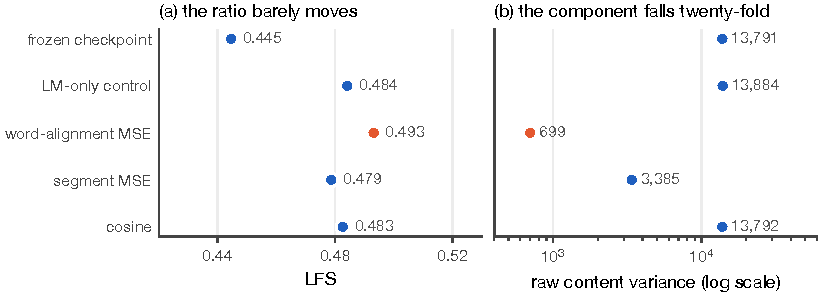
\includegraphics[width=0.7\linewidth]{fig17_ratio_hides_scale.pdf}
\end{center}
\caption{Five training conditions on Qwen3-0.6B. (a) LFS separates the shrunk
word-alignment condition from the cosine condition by 0.01. (b) Raw content variance
separates them by a factor of twenty.}
\label{fig:ratio}
\end{figure}

\section{Complementary diagnostics}
\label{app:family}
Table~\ref{tab:family} lists the diagnostics computed on the same grid as LFS, the question each answers, and what it exposes.
\begin{table}[h]
\caption{The intrinsic measures used in this paper. MEXA \citep{kargaran2024mexa} is an external retrieval-based measure reported alongside for reference.}
\label{tab:family}
\begin{center}
\small
\begin{tabular}{p{4.2cm}p{4.0cm}p{3.6cm}}
\toprule
Question & Measure & What it exposes \\
\midrule
Language vs.\ sentence-component share, per layer & LFS profile; dip depth & structure; family differences \\
Did magnitude or content variance shrink? & raw $\SSl$, $\SSc$, residual, norm vs.\ frozen reference & shrinking a ratio hides \\
Is the cross-language map simple? & nested maps M0--M5, held-out error reduction & additive vs.\ rotational vs.\ nonlinear \\
Does an English donor or a multilingual average predict a language better? & held-out $R^2$, English vs.\ average of others & English-centricity \\
Do the hardest sentences align? & AaR@10, worst-decile margin & tail failures means hide \\
\bottomrule
\end{tabular}
\end{center}
\end{table}

\section{Extended related work}
\label{app:related}
A second literature sweep (September 2026) surfaced the works below, grouped by theme. Each entry states what the work measured or did and how it relates to the present measurement.

\paragraph{Methodological sources.} The decomposition is the balanced two-way analysis of variance \citep{fisher1925}. Factor attribution and out-of-sample validation practices from empirical finance motivated the reporting conventions: variance shares of systematic factors \citep{ross1976apt,fama1993factors}, a worst-decile tail statistic \citep{artzner1999coherent,rockafellar2000cvar}, covariate adjustment of an association \citep{sharpe1966,jensen1968}, predictions frozen before held-out tests \citep{bailey2014deflated,bailey2014pseudo,lopezdeprado2018}, and the expectation that a ratio used as an objective will be gamed \citep{goodhart1975,strathern1997}; the implemented statistics are the standard ones. Mean-pooled alignment losses \citep{liu2025middle,bu2025alignx} optimize such scores directly; \S\ref{sec:stress} shows they can rise while representation magnitude shrinks.

\paragraph{Language-neutral and language-specific components, layerwise readouts, and interventions.}
\citet{kojima2024neurons} located language-specific neurons in decoder LLMs concentrated in the first and last layers and switched the output language by intervening on fewer than one percent of them; the LFS depth profile, high at both ends with an interior minimum, is a whole-representation measure of the same layout that needs neither unit selection nor generation and is comparable across models of different width.

\citet{lopo2025surgery} report that middle layers separate language-specific from language-neutral information and use a single middle-layer latent injection to control the output language; LFS quantifies one aspect of that separation, the additive main-effect share, per layer across 33 models and links it behaviorally to cross-lingual content transfer.

\citet{zhong2025think} used a logit-lens decode to show that Llama 2 relies on English alone as its internal latent language while the Japanese-adapted Swallow and LLM-jp activate both Japanese and English, so the internal language layout follows the training recipe; LFS reaches a related conclusion without decoding, since dip depth across 33 models tracks training recipe more than parameter count.

\citet{zeng2025converging} tracked BLOOM and LLaMA 2 checkpoints and found that activation similarity for translation pairs grows with training and scale while key linguistic neurons concentrate in the first and last layers; LFS summarizes the same endpoint structure as one per-layer scalar on final checkpoints across 17 primary and 19 expansion models, with a dip depth that varies with training recipe.

\citet{cheng2025abstraction} showed that intrinsic dimension peaks in the middle layers of English language models, marking the first full linguistic abstraction of the input and the layers that transfer best; LFS never estimates dimension, but its interior minimum with endpoint recovery places the layers with the smallest language share in the same region.

\citet{kriegeskorte2019onion} review representational models in systems neuroscience, including pattern component modeling, which characterizes activity patterns by the second-moment structure attributable to experimental factors; the LFS split of standardized variance into language and content sums of squares is a closed-form relative of that partition, applied to deterministic hidden states with uncertainty from sentence and model bootstraps rather than from a noise model.

\citet{conneau2020emerging} showed that jointly trained multilingual encoders develop shared cross-lingual structure even without a shared vocabulary and that separately trained monolingual models can be linked by a learned linear map, which motivates our decomposition of language variation into an additive offset plus a linear component in the misalignment decomposition.

\citet{tang2024neurons} locate language-specific feed-forward neurons by activation-probability entropy and find them concentrated in the first and last layers of decoder LLMs; LFS attributes the two main-effect sums of squares to language versus sentence identity without selecting or deactivating any unit, and its endpoint recovery places the language share at the same two extremes.

\citet{gaschi2023alignment} report that word-level alignment measured on encoder hidden states correlates with cross-lingual transfer across languages, models, and seeds, an earlier validation of an intrinsic measure against behavior; their alignment is a pairwise retrieval accuracy between English and one target language, whereas LFS is a joint variance decomposition over 128 languages with no pivot language and no word alignment.

\citet{zhang2024regions} located a core parameter region of about one percent of the weights that carries linguistic competence across 30 languages, alongside distinct monolingual regions, and showed that freezing the core region during continued pretraining limits forgetting; that localization lives in parameter space through gradient-based importance, whereas LFS lives in activation space per layer and makes no claim about which parameters carry language identity, so region-selective training is a training option that LFS can monitor but does not prescribe.

\citet{brinkmann2025grammatical} found that grammatical number, gender and tense are encoded in feature directions shared across many languages in Llama-3-8B and Aya-23-8B and confirmed the sharing by ablation; such shared content variance is what the content sum of squares in LFS is meant to capture, although LFS aggregates all matched-translation content variance into one share and never labels individual concepts.

\citet{bandarkar2025swapping} composed a multilingual reasoner by taking the top and bottom layers from a target-language expert and the middle layers from an English math expert, gaining about ten percent on MGSM without target-language task data; the recipe presupposes the layer geography that LFS measures, language at the endpoints and content in the interior, and an LFS profile could inform where the transition zone is placed.

\paragraph{Measurement geometry, standardization, and calibration.}
\citet{rudman2022isoscore} showed that common isotropy measures such as the average random cosine and the partition score are brittle and overturned several published conclusions that rested on them; LFS therefore fixes coordinate scale by a single joint per-coordinate z-scoring before asking what share of the two main-effect sums of squares language identity carries, and treats that standardization as a stated measurement decision rather than a tuned one.

\citet{hammerl2023anisotropy} studied outlier dimensions and anisotropy in multilingual encoders and compared outlier removal, cluster-based isotropy enhancement, and ZCA whitening as ways to raise cross-lingual similarity; LFS applies one fixed joint per-coordinate standardization as measurement preprocessing and never tunes it to a downstream score, which is what lets the content-variance preservation check detect a collapse that similarity-style measures miss.

\citet{chi2021infoxlm} framed cross-lingual pretraining as maximizing mutual information across translation views and introduced the contrastive objective that our contrastive training condition instantiates; LFS is defined without any training signal, as the language main effect's share of the two main-effect sums of squares, and serves here to read what that objective did to the representation.

\citet{tiyajamorn2021representation} model a multilingual sentence embedding as the sum of a meaning vector and a language vector and train a module to remove the latter for similarity estimation; LFS reads the same additive partition directly from the variance of matched translations at every layer, without training any component.

\citet{kim2026langsae} remove language identity from retrieval embeddings post hoc with a sparse autoencoder and compare against centering and All-but-the-Top; such methods choose how much language signal to delete, whereas LFS reports how much is present and, through the collapse blind spot, shows that removal can hide a loss of content variance.

\citet{miller2024evals} gives standard-error formulas for eval accuracy, paired model comparisons, and clustered items, treating an evaluation as an experiment with an explicit sampling unit; we take sentences within a model as the unit for the LFS half-widths and models across 13 families as the unit for the interval on the LFS-to-$R_{\mathrm{content}}$ association.

\citet{ethayarajh2019contextual} showed that contextual representations are anisotropic in every layer and that the degree of anisotropy changes with depth, so comparing a variance partition across layers requires removing shared scale first, which is the role of the joint per-coordinate z-scoring that precedes $\mathrm{SS}_{\mathrm{lang}}$ and $\mathrm{SS}_{\mathrm{con}}$.

\citet{kovaleva2021outlier} document a handful of high-magnitude outlier dimensions that dominate hidden-state statistics in pretrained transformers; without per-coordinate standardization these dimensions would dominate both sums of squares in LFS and would also inflate raw-variance measures such as the content-variance preservation check.

\citet{sun2024massive} show that decoder LLMs, including the Llama and Mistral families in our grid, carry a few input-independent activations up to 100,000 times larger than the rest that act as bias terms; such fixed-dimension constants are identical across grid cells, contribute no centered variance to either main effect, and distort raw norm measures, which is why coordinates are standardized before the partition and the norm-shrinkage measure is reported separately.

\citet{hewitt2019control} showed that probe accuracy can reflect probe capacity rather than encoded information and introduced random-label control tasks to calibrate it; LFS has no trained component, so its calibration is analytic, the pure-noise value $(L-1)/(L+N-2)=0.298$ that follows from the degrees of freedom of the two main effects.

\citet{wang2020uniformity} show that the contrastive loss acts on L2-normalized features and decomposes into an alignment term and a uniformity term, which is the formal reason a cosine or InfoNCE objective is invariant to representation norm and cannot register the 451-to-42 norm shrinkage that only the norm and the raw content-variance measure detected.

\citet{yang2021bias} found that the leading principal components of a weakly aligned multilingual encoder mostly encode language identity and removed them by orthogonal projection to improve retrieval; LFS leaves the geometry intact and instead reports the language main effect's share of variance at each layer after joint per-coordinate z-scoring, which is not a count of dimensions.

\citet{rajaee2022isotropy} showed that mBERT is strongly anisotropic with language-specific dominant directions rather than shared outlier dimensions, and that removing those directions per language improves semantic tasks; LFS therefore z-scores every coordinate jointly across the language grid so that a few high-variance coordinates cannot dominate the language share, and then measures rather than repairs.

\citet{belrose2023tuned} showed that per-layer vocabulary readouts from the logit lens are brittle and become reliable only after an affine probe is fitted for each block; LFS reads layer geometry directly from z-scored hidden states as a closed-form variance ratio and needs neither a fitted probe nor a vocabulary projection.

\citet{kreutzer2025dejavu} argued that multilingual LLM evaluation should adopt the meta-evaluation, significance testing and transparent reporting practices developed for machine translation; the protocol here follows that advice through preregistration, sentence and model bootstraps and a FLORES-200 replication, while LFS itself is an intrinsic measure whose behavioral checks are a translation-based content-transfer measure and the paired Belebele null.

\citet{godey2024anisotropy} showed that anisotropy is a general property of transformer hidden states across training objectives and modalities, including decoder language models like those in our grid, and traced its cause to the query and key spaces of self-attention; LFS does not model the cause and instead removes shared per-coordinate scale by joint z-scoring before asking how much of the remaining variance is attributable to language identity.

\citet{puccetti2022outlier} linked the magnitude of outlier dimensions to token frequency in pretraining data and to attention on special tokens; because token frequency differs sharply across languages, this is nuisance variance that could pass for language signal in an unstandardized partition, so LFS removes per-coordinate scale before the variance partition and leaves the frequency-to-language confound as a stated limitation.

\paragraph{Data and evaluation protocol.}
\citet{bagherinezhad2024drives} explained per-language accuracy on SIB-200 across 204 languages by pretraining data size for seen languages and by script and language family for unseen ones; the confound removal uses the same covariates, and the per-language $\mathrm{SS}_{\mathrm{lang}}$ shares at the dip let us ask whether the above-uniform Arabic and Persian shares are a data-size or a script effect.

\citet{skean2025layer} show with entropy, geometry, and invariance measures across transformer and state-space models that intermediate layers carry the strongest representations for downstream embedding tasks, which supports reading the behavioral predictor $1-\mathrm{LFS}$ at the dip layer rather than at the final layer.

\citet{artetxe2020artifacts} show that human and machine translation leave artifacts that shift XNLI accuracy by several points; our WMT19 check finds that translated text carries a slightly higher language share than native text (+0.02 to +0.06) with the cross-model ordering unchanged (Spearman 0.99), so in that panel translationese shifted the level and left the ordering unchanged.

\citet{rust2021tokenizer} introduced tokenizer fertility and the proportion of continued words as diagnostics and showed that, together with pretraining data size, they explain much of the gap between multilingual and monolingual models; fertility depends on the tokenizer, the text, and the word-count convention, and enters our covariate set because LFS is computed on mean-pooled hidden states, whose pooling length and vocabulary coverage it affects; we do not claim these are its only routes.

\paragraph{Validation, confounds, collapse, and training objectives.}
\citet{gonen2020greek} showed on mBERT that subtracting a language's mean token vector and adding another's moves nearest neighbors onto translations, a qualitative intervention on one encoder that implies an additive language component; the misalignment decomposition quantifies that component without intervening, finding that 63 to 97 percent of the cross-language misalignment is an additive shift plus isotropic scale across 128 languages.

\citet{zhao2021inducing} evaluated re-centering, re-alignment of each language's space to a pivot, and input normalization as ways to remove language-specific statistics from encoder representations and scored them by the cross-lingual transfer gap; LFS alters nothing and instead reports, per layer, how much of the two main-effect variances language identity still accounts for, so it is a measure that can be taken before and after such repairs rather than a repair itself.

\citet{zhao2025disentanglement} projected a language-specific subspace out of hidden states at inference time and reported improved multilingual reasoning on ten open-weight models; LFS neither intervenes nor optimizes, and its pooled Belebele null across 33 models after confound removal indicates that the size of the language share on its own does not predict benchmark accuracy, so the two measures answer different questions.

\citet{deng2025unveiling} found sparse-autoencoder features tied to single languages whose ablation removes that language alone, evidence that language identity occupies a small set of additive directions; the LFS misalignment decomposition, in which 63 to 97 percent of the cross-language misalignment is an additive shift plus isotropic scale, is a closed-form counterpart that requires no learned dictionary and so cannot name features but also cannot inherit dictionary training choices.

\citet{lauscher2020hero} showed that zero-shot transfer with multilingual transformers degrades with smaller target-language pretraining corpora and greater linguistic distance from the source; LFS predicts $R_{\mathrm{content}}$ from hidden states alone with no language metadata, and the confound-removal analysis asks whether these two covariates explain the association away.

\citet{ali2024tokenizer} trained 24 monolingual and multilingual 2.6B models under different tokenizers and found that fertility and parity do not reliably predict downstream accuracy, so fertility enters the LFS confound removal as one regressor among several rather than as a sufficient control for tokenizer effects.

\citet{wu2025bitter} surveyed more than 2,000 multilingual benchmarks and found that a localized benchmark agrees with human judgments at 0.68 while translated versions of the same benchmark reach about 0.47, with task-level agreement ranging from 0.11 to 0.85; this spread in criterion validity is one reason a pooled Belebele benchmark criterion can be null for LFS while the content-transfer criterion is not.

\citet{idris2026embedding} found across 816 transfer experiments on African languages that cosine-gap and retrieval-based similarity predict transfer within each model (Spearman 0.37 to 0.60 for NER) while the correlation pooled across models turns negative and CKA carries little signal; the model-level bootstrap interval in the LFS validation, [0.19, 0.71] over 19 models from 13 families, is reported because of this pooling hazard; it quantifies uncertainty under model resampling and does not by itself remove model-level confounding.

\citet{ding2021grounding} argued that a representation measure should respond to changes that alter function and ignore those that do not, and showed that CKA and CCA each fail on one side; the LFS validation follows this logic with a behavioral target (cross-lingual content transfer), a pooled-accuracy null on Belebele, a known pure-noise value of 0.298, and sentence and model bootstraps.

\citet{bardes2022vicreg} prevent collapse in self-supervised learning with a hinge penalty on the per-dimension standard deviation of embeddings, paired with an invariance term of matched scale; the CVP penalty in our training conditions is a different object, a squared hinge on an aggregate content-variance ratio; attached to a pretrained LLM alongside the alignment term it saturated at every weight tested and did not prevent the contraction, which is why CVP is used here as a measure rather than as an objective.

\citet{ji2024emma} continued pretraining Llama 2 7B on the MaLA corpus across 546 languages and reported gains for low-resource languages; LFS changes nothing in a model, but taken before and after such continued pretraining it can quantify how the intervention reshapes the language-identity depth profile.

\citet{gao2023scaling} showed that optimizing a proxy reward too hard lowers the gold objective with a smooth and predictable functional form; the corresponding failure for LFS is a sign reversal rather than a gradual decline, since minimizing it as a training loss flipped its observational association with tail alignment (Pearson +0.924 across 18 condition-seed points), which is why LFS is reported as a measurement; it was tested as an objective and is not recommended as one.

\citet{huang2024erasure} train dense retrievers with a linear concept-erasure loss that penalizes correlation between embeddings and language labels and report retrieval gains; our collapse experiment shows that retrieval measures can improve while raw content variance shrinks, which is why LFS is kept as a measurement rather than a training target.

\citet{sterz2025recover} steer generation toward a target language by adding or subtracting per-language mean activations estimated from a multi-parallel corpus; the dominance of the additive offset plus a scale in our misalignment decomposition, 63 to 97 percent of the held-out cross-language misalignment, is consistent with their finding that mean-difference steering works at intermediate layers.

\citet{harrasse2025transcoders} report with cross-layer transcoders that early layers use highly similar sparse features across languages while language-specific decoding features appear late; feature overlap and variance share answer different questions, so an early layer can show shared features and still carry the high language-variance share that LFS reports, driven by token and script identity.

\citet{korner2026meanings} use activation patching across EuroLLM pretraining checkpoints to show that shared concept spaces emerge early in training with alignment quality that varies by language; LFS is observational and covers final checkpoints of 17 model families, and in EuroLLM, Persian carries an above-uniform language share at the dip while Arabic does not (Table~\ref{tab:focal_share}).

\citet{singh2025globalmmlu} find that 28 percent of MMLU items require culturally specific knowledge and that model rankings shift between culturally sensitive and culturally agnostic subsets, so pooled translated-benchmark accuracy is a noisy criterion; this frames our null result for LFS against pooled Belebele accuracy after confound removal and our use of content transfer as the matched criterion.

\citet{cao2020alignment} fine-tune mBERT with a parallel-data alignment loss on matched contextual word representations and judge success by contextual word retrieval and zero-shot XNLI; the word-alignment objective we tested follows this recipe, and under it representation norm fell from 451 to 42 while retrieval measures improved and LFS moved from 0.445 to 0.493, so the norm and the raw content-variance measure, not the ratio, caught the contraction.

\citet{conneau2020unsupervised} describe the curse of multilinguality, the trade-off at fixed capacity between positive transfer and per-language dilution measured in downstream accuracy; LFS instead describes where language identity lives in the depth profile, and the finding that dip depth tracks training recipe more than size, together with the null result for code-switched training, sits on the representation side of that trade-off.

\citet{dasilva2025steering} evaluate three activation-steering methods on 36 models from 14 families and find that many models show no downstream improvement or degrade, a reliability failure for inference-time interventions that parallels the negative results for training-time interventions in our stress tests, and our multi-family model bootstrap addresses the same few-model-generalization concern from the measurement side.

\citet{yan2023bleurt} show that training an MT system directly against BLEURT by minimum risk training produces degenerate universal translations that the metric scores highly, a measurement-versus-objective failure familiar to the MT community; the reversal of the LFS association when LFS was minimized as a loss is the representation-level analogue and is why LFS stays a measurement.

\citet{schut2025english} used the logit lens and activation steering on French, German, Dutch and Mandarin inputs to show that key semantic decisions are taken in an English-like intermediate representation and that steering vectors computed in English transfer better than vectors computed in the input language; our English-hub test asks a complementary question across 127 languages and finds that a multilingual latent factor predicts each language better than English does for 113 to 124 of them.

\citet{zhong2026sparse} located the transition from English-aligned intermediate representations back to target-language token space in a small set of dimensions at consistent indices and switched the output language by editing them while preserving content; LFS treats all coordinates symmetrically after z-scoring and reports an aggregate per-layer share with an additive-offset decomposition, so it makes no claim about whether the language component is sparse.

\citet{wu2020equal} showed that within-language quality in mBERT falls sharply for languages with little pretraining data, with NER on 99 languages and POS tagging and parsing on 54; this data-size confound is why the pooled Belebele analysis partials out pretraining share before reading the LFS association, which is then null on 33 models.

\citet{wang2024emergence} tracked a neuron-overlap alignment measure across BLOOM pretraining checkpoints and found that it correlates with zero-shot transfer while passing through non-monotone phases; LFS is read once per released model across 17 families rather than along a training run, so the checkpoint at which a measure is taken is a stated limitation, and their probe-based measure differs from the probe-free variance ratio used here.

\citet{ki2025nepotism} show that multilingual retrieval-augmented generation systems sometimes cite documents for their language rather than their relevance across eight languages and six models, a behavioral form of language preference that an intrinsic measure of hidden-state structure does not address directly.

\citet{alali2026english} compared 27 cross-lingual alignment score variants as predictors of classification and translation quality and found that alignment with English predicts translation quality about as well as source-target alignment; their scores are pairwise similarities with English as pivot, whereas LFS is a joint decomposition over 128 languages with no pivot, and our English-hub test finds that a multilingual latent factor predicts each language better than English does for 113 to 124 of 127 languages.

\citet{davari2023cka} showed that CKA is sensitive to outliers and to translations of a subset of the representations, and that representations can be edited to move the CKA value while the network's function is unchanged; LFS is a single-representation variance partition over a language grid with an analytic pure-noise value of 0.298 rather than a pairwise similarity, and the analogous manipulability appears in our experiments only when LFS is minimized directly as a training objective, where its observational association reverses.

\citet{belinkov2022probing} reviewed probing classifiers and showed that probe capacity, the gap between correlation and causation, and low selectivity all confound what a probe appears to read out; LFS requires no fitted probe: it is a parameter-free variance partition that needs only matched translations and a layer index, and the paper pairs it with intervention-style stress tests and a behavioral prediction rather than resting on encoded-property claims alone.

\citet{wu2020explicit} proposed a contrastive alignment objective for mBERT and XLM-R and then found, under a more careful evaluation, that explicit alignment objectives do not improve downstream transfer and are eclipsed by a stronger underlying model; they judged alignment only by downstream accuracy, while the null LFS association with pooled benchmark accuracy on 33 models and its positive association with content transfer on 19 models make a related point from the representation side.

\citet{jing2022collapse} showed that contrastive objectives can drive embeddings into a low-dimensional subspace through strong augmentation and implicit regularization, diagnosing the collapse from the embedding covariance spectrum; the word-alignment condition shows a related but weaker pattern in a multilingual LLM, a magnitude contraction with raw content variance falling from 13,791 to 699 while LFS moved only from 0.445 to 0.493 (the spectrum was not measured, so no loss of rank is claimed), which is why the paper pairs LFS with a content-variance preservation check.

\citet{chang2024curse} trained more than 10,000 small controlled models and found that moderate multilingual data helps low-resource languages while high-resource languages consistently lose, with gains depending on syntactic similarity; this gives quantitative context for the monotone cost on unseen languages observed under code-switched training, though LFS is computed on frozen hidden states of released models and does not itself prescribe a data mixture.

\citet{sundar2025steering} showed that finding-experts activation interventions reshape a multilingual LLM's embedding space and raise cross-lingual retrieval top-1 accuracy by up to a factor of two; retrieval is exactly the measure that improved in our word-alignment condition while representation norm and raw content variance collapsed, which is why LFS is paired with a raw content-variance check rather than read alongside retrieval alone.

\citet{she2024mapo} built a DPO or PPO preference signal from translation-model consistency between answers in non-dominant and dominant languages and reported stable multilingual reasoning gains, which is a preference-training approach to the same problem; MAPO aligns behavior through preferences over generated answers and is scored on reasoning accuracy, whereas LFS measures hidden-state geometry and is null on pooled benchmark accuracy, so the two address different levels of the alignment question.

\section{Corrections ledger}
\label{app:ledger}
Every discrepancy found during the project is recorded with its date, cause, and fix in a ledger shipped with the code. In summary: a torn line in the run ledger (file locking added); a stale prototype result left in a results directory (renamed so that globs fail loudly); a size-invariance claim stated too strongly (replaced by the exact expected value and its verifications); a permutation-null criterion written with an inverted inequality (corrected before scoring); function words contaminating a word-level concept grid (filtered at the concept definition); an Aim-2 collapse criterion that the control condition also failed (criterion rewritten); a criterion scored on sign alone (replaced by an effect-size criterion); a preregistration that mis-described its own held-out set (left as written, with the correction attached); an inert variance-preservation term in the word-level trainer (fixed and rerun); a frozen reference skipped by name in an evaluation script (identified by set membership instead); profile counts that combined the two estimators (reported separately since); a hub result stated as universal when it is model-specific (reported as a range); and, during the final revision, a regression statistic cited from the development-grid run rather than the 17-model artifact (corrected in \S\ref{sec:setup} and Appendix~\ref{app:deflation}), and an offset-plus-scale range quoted from a three-model prototype at selected ranks (65 to 98 percent) where the 14-model common-rank artifacts give 63 to 97 percent (corrected throughout).

\section{Six focal languages}
\label{app:focal}
Each analysis uses its full prespecified language support (128 on the grid, 116 on FLORES-200, 41 on the content-transfer test with 34 in the common-support summary, 24 in the language probe, 40 and 70 in the benchmark panels); no language was selected or removed after outcomes. For readers who want a fixed set to follow through the
paper, Tables~\ref{tab:focal_rcontent} and \ref{tab:focal_share} report six
high- and mid-resource languages spanning three scripts (Latin, Cyrillic, and Arabic): German, French,
Spanish, Russian, Arabic, and Persian.
\begin{table}[h]\caption{Content transfer $R_{\mathrm{content}}$ (matched minus mismatched context benefit, normalized by English) for the six focal languages across the 19 frozen models of the expansion set.}\label{tab:focal_rcontent}
% ---- table focal_rcontent (inlined) ----
\begin{center}\scriptsize
\begin{tabular}{lrrrrrr}
\toprule
Model & German & French & Spanish & Russian & Arabic & Persian \\
\midrule
Falcon3-3B-Base & 0.60 & 0.77 & 0.78 & 0.30 & 0.04 & 0.13 \\
Llama-3.1-8B & 0.79 & 0.76 & 0.74 & 0.69 & 0.62 & 0.66 \\
Mistral-Nemo-Base-2407 & 0.77 & 0.79 & 0.78 & 0.72 & 0.68 & 0.65 \\
OLMo-2-1124-13B & 0.75 & 0.76 & 0.79 & 0.62 & 0.48 & 0.56 \\
Qwen2.5-0.5B & 0.59 & 0.68 & 0.69 & 0.54 & 0.45 & 0.32 \\
Qwen2.5-1.5B & 0.69 & 0.71 & 0.70 & 0.61 & 0.53 & 0.46 \\
Qwen2.5-3B & 0.69 & 0.73 & 0.73 & 0.65 & 0.60 & 0.53 \\
Qwen2.5-7B & 0.77 & 0.75 & 0.73 & 0.69 & 0.64 & 0.63 \\
Sailor-1.8B & 0.60 & 0.67 & 0.66 & 0.47 & 0.28 & 0.22 \\
Sailor-7B & 0.74 & 0.73 & 0.75 & 0.65 & 0.54 & 0.50 \\
SmolLM2-360M & 0.51 & 0.60 & 0.59 & 0.22 & 0.05 & 0.11 \\
TowerBase-7B & 0.73 & 0.78 & 0.77 & 0.68 & 0.43 & 0.44 \\
Yi-1.5-9B & 0.71 & 0.75 & 0.73 & 0.59 & 0.46 & 0.46 \\
granite-3.1-8b-base & 0.74 & 0.70 & 0.72 & 0.55 & 0.51 & 0.44 \\
mGPT & 0.79 & 0.77 & 0.77 & 0.67 & 0.52 & 0.56 \\
occiglot-7b-eu5 & 0.82 & 0.78 & 0.78 & 0.61 & 0.36 & 0.34 \\
xglm-1.7B & 0.69 & 0.69 & 0.72 & 0.59 & 0.48 & 0.23 \\
xglm-2.9B & 0.72 & 0.72 & 0.73 & 0.62 & 0.55 & 0.25 \\
xglm-7.5B & 0.73 & 0.75 & 0.76 & 0.66 & 0.58 & 0.27 \\
\bottomrule
\end{tabular}
\end{center}

\end{table}
\begin{table}[h]\caption{Share of the language sum of squares $\SSl$ carried by each focal language at the dip layer (1,500-sentence dumps, 14 models). A uniform share would be $1/128 = 0.0078$; a language above it contributes more than its share of the language component.}\label{tab:focal_share}
% ---- table focal_langshare (inlined) ----
\begin{center}\scriptsize
\begin{tabular}{lrrrrrrr}
\toprule
Model & German & French & Spanish & Russian & Arabic & Persian & Uniform share \\
\midrule
EuroLLM-1.7B & 0.0041 & 0.0040 & 0.0041 & 0.0042 & 0.0046 & 0.0094 & 0.0078 \\
Falcon3-7B-Base & 0.0065 & 0.0079 & 0.0082 & 0.0068 & 0.0062 & 0.0068 & 0.0078 \\
Mistral-7B-v0.3 & 0.0058 & 0.0048 & 0.0050 & 0.0048 & 0.0096 & 0.0104 & 0.0078 \\
OLMo-2-0425-1B & 0.0065 & 0.0060 & 0.0053 & 0.0054 & 0.0057 & 0.0052 & 0.0078 \\
OLMo-2-1124-7B & 0.0058 & 0.0057 & 0.0052 & 0.0049 & 0.0042 & 0.0044 & 0.0078 \\
Qwen3-0.6B-Base & 0.0060 & 0.0059 & 0.0059 & 0.0058 & 0.0069 & 0.0051 & 0.0078 \\
Qwen3-1.7B-Base & 0.0062 & 0.0056 & 0.0055 & 0.0054 & 0.0068 & 0.0056 & 0.0078 \\
Qwen3-4B-Base & 0.0058 & 0.0055 & 0.0055 & 0.0052 & 0.0063 & 0.0049 & 0.0078 \\
Qwen3-8B-Base & 0.0052 & 0.0049 & 0.0051 & 0.0049 & 0.0061 & 0.0048 & 0.0078 \\
SmolLM2-1.7B & 0.0064 & 0.0055 & 0.0052 & 0.0061 & 0.0065 & 0.0062 & 0.0078 \\
bloom-1b7 & 0.0060 & 0.0048 & 0.0047 & 0.0073 & 0.0055 & 0.0054 & 0.0078 \\
bloom-7b1 & 0.0053 & 0.0042 & 0.0042 & 0.0061 & 0.0045 & 0.0057 & 0.0078 \\
salamandra-2b & 0.0060 & 0.0039 & 0.0059 & 0.0047 & 0.0121 & 0.0104 & 0.0078 \\
salamandra-7b & 0.0044 & 0.0043 & 0.0045 & 0.0045 & 0.0086 & 0.0110 & 0.0078 \\
\bottomrule
\end{tabular}
\end{center}

\end{table}

\end{document}
